% ============================================================================
% Master's defence — Universal Properties from Quantum Many-Body Dynamics
% Joaquín G. Márquez Olguín · supervisor Stefano Carignano (BSC)
%
% Build, from this directory:
%   tectonic -X compile main.tex --outfmt pdf -Z shell-escape
% ============================================================================
\documentclass[aspectratio=169,11pt]{beamer}

\usepackage[british]{babel}
\usepackage[T1]{fontenc}
\usepackage{lmodern}
\usepackage{amsmath,amssymb,bm}
\usepackage{bbold}     % blackboard-bold digits: \mathbb{1} as in the thesis
% bbold ships only a few design sizes; map every size onto bbold10 so that
% \mathbb{1} does not fall back to a missing font at 11pt and above
\DeclareFontFamily{U}{bbold}{}
\DeclareFontShape{U}{bbold}{m}{n}{<->bbold10}{}
\usepackage{graphicx}
\usepackage{booktabs}
\usepackage{tikz}
\usetikzlibrary{patterns,calc,shapes.geometric}
\usepackage{animate}   % GIF-in-PDF for the dual-unitarity circle (plays in Acrobat)
\graphicspath{{imgs/}{../thesis/imgs/}}

% ---- palette, taken from the PowerPoint template -----------------------------
\definecolor{ink}{RGB}{31,42,54}       % text, frame titles
\definecolor{accent}{RGB}{5,141,199}   % structure, taglines
\definecolor{blob}{RGB}{169,220,235}   % background gradients
\definecolor{hl}{RGB}{196,98,22}       % orange highlights only
% colours of the fermionised Hamiltonian terms (backup B1), matching the FSM figure
\definecolor{jwnn}{RGB}{40,80,150}
\definecolor{jwfield}{RGB}{40,130,70}
\definecolor{jwnnn}{RGB}{150,60,150}
\definecolor{jwxx}{RGB}{196,98,22}
% the two routes to c, used as soft background bands on every results slide.
% deliberately outside the term colours above so the two systems never collide:
\definecolor{routeV}{RGB}{17,122,101}   % entropy route  -- the eigenVectors
\definecolor{routeL}{RGB}{162,59,114}   % spectral route -- the eigenvaLues
\definecolor{warn}{RGB}{176,58,46}      % "beyond here the simulation is wrong"

\setbeamercolor{normal text}{fg=ink,bg=white}        % body text on white
\setbeamercolor{structure}{fg=accent}                % "structure" = bullets, enum numbers, etc.
\setbeamercolor{frametitle}{fg=ink,bg=}              % slide titles: dark ink, NO coloured bar (empty bg)
\setbeamercolor{title}{fg=ink,bg=}                   % (title-page slot; we build ours by hand anyway)
\setbeamercolor{block title}{bg=accent!10,fg=accent!80!black}  % \begin{block} header tint
\setbeamercolor{block body}{bg=accent!4,fg=ink}                % \begin{block} body tint
\setbeamertemplate{navigation symbols}{}             % kill the tiny nav icons Beamer adds by default
\setbeamertemplate{blocks}[rounded][shadow=false]    % rounded blocks, flat (no fake 3D shadow)
\setbeamerfont{frametitle}{series=\bfseries,size=\large}
% bullet symbols, drawn in the accent colour:
\setbeamertemplate{itemize item}{\textcolor{accent}{\raisebox{0.12ex}{\scriptsize$\blacktriangleright$}}}
\setbeamertemplate{itemize subitem}{\textcolor{accent!70}{--}}

% ---- background: white with soft cyan blobs in the corners -------------------
% \bgblobs is the default, \bgtitle is swapped in for the title slide alone.
% The paper is 160 x 90 mm at aspectratio=169; coordinates below are in cm, and
% the blobs must stay pushed off the corners or the white boxes of the plot PDFs
% cut visibly into them.
\newcommand{\bgblobs}{% content frames: subtle, pushed into the corners
  
\begin{tikzpicture}
    \useasboundingbox (0,0) rectangle (16,9);
    \shade[shading=radial, inner color=blob!50, outer color=white]
      (16.2,9.2) circle (2.1);
    \shade[shading=radial, inner color=blob!35, outer color=white]
      (-0.2,-0.2) circle (1.9);
  \end{tikzpicture}}
\newcommand{\bgtitle}{% title frame: larger blobs, uniform background
  
\begin{tikzpicture}
    \useasboundingbox (0,0) rectangle (16,9);
    \shade[shading=radial, inner color=blob!85, outer color=white]
      (13.6,7.9) circle (4.0);
    \shade[shading=radial, inner color=blob!60, outer color=white]
      (0.9,0.7) circle (3.0);
  \end{tikzpicture}}
\setbeamertemplate{background}{\bgblobs}

% ---- frame title: ink, left, short accent rule, section tag on the right -----
% \slidesection{...} sets the small tag printed at the right of the title, so a
% listener always knows which part of the talk they are in. It stays set until
% changed, so it is written once per section, not once per frame. \nosection
% clears it (title slide, thank-you slide).
\newcommand{\thesectiontag}{}
\newcommand{\slidesection}[1]{\renewcommand{\thesectiontag}{#1}}
\newcommand{\nosection}{\renewcommand{\thesectiontag}{}}
\setbeamertemplate{frametitle}{%
  \vspace*{0.42cm}%
  \begin{minipage}[b]{0.685\textwidth}\raggedright
    \usebeamerfont{frametitle}\usebeamercolor[fg]{frametitle}\insertframetitle
  \end{minipage}\hfill
  \begin{minipage}[b]{0.295\textwidth}\raggedleft
    \normalfont\mdseries\footnotesize\color{accent!55}\thesectiontag
  \end{minipage}\par
  \vspace*{0.08cm}%
  {\color{accent}\rule{2.6cm}{1.5pt}}\par\vspace*{-0.05cm}}

% ---- footer: name | short title | page (hidden for backup frames) ------------
% \inappendixtrue is set just before the backup frames; the footer then prints
% "backup" in place of the page number. Three coloured boxes in the Madrid
% style, rebuilt by hand to keep that behaviour and this palette.
\newif\ifinappendix
\definecolor{footnavy}{RGB}{31,64,110}
\setbeamercolor{author in head/foot}{bg=footnavy,fg=white}
\setbeamercolor{title in head/foot}{bg=footnavy!75!white,fg=white}
\setbeamercolor{date in head/foot}{bg=footnavy!55!white,fg=white}
\setbeamertemplate{footline}{%
  \leavevmode%
  \hbox{%
\begin{beamercolorbox}[wd=.24\paperwidth,ht=2.4ex,dp=1.1ex,center]{author in head/foot}%
    \usebeamerfont{author in head/foot}\scriptsize Joaquín G. Márquez
  \end{beamercolorbox}%
\begin{beamercolorbox}[wd=.52\paperwidth,ht=2.4ex,dp=1.1ex,center]{title in head/foot}%
    \usebeamerfont{title in head/foot}\scriptsize Universal Properties from Quantum Many-Body Dynamics\strut%
  \end{beamercolorbox}%
\begin{beamercolorbox}[wd=.24\paperwidth,ht=2.4ex,dp=1.1ex,right]{date in head/foot}%
    \usebeamerfont{date in head/foot}\scriptsize September 2026\hspace*{1.6em}
    \ifinappendix backup\else\insertframenumber{} / \inserttotalframenumber\fi\hspace*{2ex}
  \end{beamercolorbox}}%
  \vskip0pt}

% ---- shorthand ---------------------------------------------------------------
% Small macros so the slide source stays readable:
%   \E            the transfer matrix, \Lech the Loschmidt echo
%   \ket/\bra/\braket   Dirac notation
%   \idea{...}    the one-line "main idea" tagline (bold, accent colour)
%   \fullresults   Table 1, with a colour band per route to $c$
\newcommand{\E}{\mathcal{E}}
\newcommand{\Lech}{\mathcal{L}}
\newcommand{\Tr}{\mathrm{Tr}}
\newcommand{\ket}[1]{\left|#1\right\rangle}
\newcommand{\bra}[1]{\left\langle#1\right|}
\newcommand{\braket}[2]{\left\langle#1\middle|#2\right\rangle}
% one-line "main idea" tagline
\newcommand{\idea}[1]{\begin{center}\color{accent!80!black}\textbf{#1}\end{center}}

% ---- attribution, highlights, panels -----------------------------------------
% \src{...}  a small grey source note, placed next to the thing it supports.
%            The deck names only the handful of papers a listener would want.
\newcommand{\src}[1]{{\scriptsize\color{ink!45}#1}}
% \hlt{colour}{...}  colour a symbol or phrase, no panel.
\newcommand{\hlt}[2]{{\color{#1!85!black}#2}}
% \hlb{colour}{...}  the same, sitting on a soft translucent panel. Inline, so
%            it works inside a display equation as well as in text.
\newcommand{\hlb}[2]{%
  \tikz[baseline=(hlbX.base)]{\node[rectangle,rounded corners=2pt,
    inner xsep=3pt,inner ysep=1.5pt,fill=#1!14](hlbX){#2};}}
% \tint{colour}{...}  a rounded soft panel around a whole box (a tabular, a
%            short statement). Used for the two route bands on the results.
\newcommand{\tint}[2]{%
  \tikz[baseline=(tintX.base)]{\node[rectangle,rounded corners=3pt,
    inner sep=4pt,fill=#1!12](tintX){#2};}}
% \routelabel{colour}{...}  the tiny caption naming a route band.
\newcommand{\routelabel}[2]{{\scriptsize\color{#1!85!black}#2}}
% one cell of the entropy grid on Results I: figure + its extracted result
\newcommand{\domecell}[5]{%
  \begin{minipage}{0.487\textwidth}\centering
    \includegraphics[width=\textwidth]{#2}\\[-0.2ex]
    {\footnotesize\color{#1!85!black} $c = #3$ \ (#4,
      \ $v_\infty T =$ #5)}%
  \end{minipage}}

% ---- results tables -----------------------------------------------------------
% \fullresults: the full Table 1 (used on the Results opener and the
% conclusions). Each results slide instead shows only its own columns via the
% three mini-tables below.
\newcommand{\entropyminitable}{%
  {\centering\footnotesize\tint{routeV}{%
  \setlength{\tabcolsep}{5pt}\renewcommand{\arraystretch}{1.05}%
  \begin{tabular}{@{}ccc@{}}
  \toprule
  $p$ & window & $c$ (entropy)\\
  \midrule
  $0$   & $4\le T\le 22$ & $0.49\pm0.01$\\
  $0.1$ & $4\le T\le 13$ & $0.50\pm0.04$\\
  $0.3$ & $2\le T\le 9$  & $0.53\pm0.04$\\
  $0.5$ & $2\le T\le 5$  & $0.58\pm0.04$\\
  \bottomrule
  \end{tabular}}\par}}
\newcommand{\spectralminitable}{%
  {\centering\footnotesize\tint{routeL}{%
  \setlength{\tabcolsep}{5pt}\renewcommand{\arraystretch}{1.05}%
  \begin{tabular}{@{}ccc@{}}
  \toprule
  $p$ & window & $c$ (spectral)\\
  \midrule
  $0$   & $2\le T\le 22$ & $0.45$\\
  $0.1$ & $2\le T\le 17$ & $0.47$\\
  $0.3$ & $2\le T\le 10$ & $0.49$\\
  $0.5$ & $2\le T\le 6$  & $0.53$\\
  \bottomrule
  \end{tabular}}\par}}
\newcommand{\towerminitable}{%
  {\centering\footnotesize\tint{routeL}{%
  \setlength{\tabcolsep}{5pt}\renewcommand{\arraystretch}{1.05}%
  \begin{tabular}{@{}cc@{}}
  \toprule
  $p$ & $x_1$\\
  \midrule
  $0$   & $0.498$\\
  $0.1$ & $0.497$\\
  $0.3$ & $0.493$\\
  $0.5$ & $0.487$\\
  \bottomrule
  \end{tabular}}\par}}
% \fullresults: Table 1, split into three groups so the two routes to c can
% carry their own soft colour band -- the route colours are introduced here and
% reused on every results slide and in the conclusions.
\newcommand{\fullresults}{%
  {\centering\small
  \setlength{\tabcolsep}{6pt}\renewcommand{\arraystretch}{1.25}%
  \begin{tabular}{@{}c@{\;}c@{\;}c@{}}
    & \routelabel{routeV}{from the eigen\emph{vectors}}
    & \routelabel{routeL}{from the eigen\emph{values}}\\[0.15ex]
    \tint{white}{%
      \begin{tabular}{@{}cc@{}}
      \toprule
      $p$ & $v_\infty$\\
      \midrule
      $0$   & $2.00$\\
      $0.1$ & $2.67$\\
      $0.3$ & $3.97$\\
      $0.5$ & $5.21$\\
      \bottomrule
      \end{tabular}}
    & \tint{routeV}{%
      \begin{tabular}{@{}cc@{}}
      \toprule
      window & $c$ (entropy)\\
      \midrule
      $4\le T\le 22$ & $0.49\pm0.01$\\
      $4\le T\le 13$ & $0.50\pm0.04$\\
      $2\le T\le 9$  & $0.53\pm0.04$\\
      $2\le T\le 5$  & $0.58\pm0.04$\\
      \bottomrule
      \end{tabular}}
    & \tint{routeL}{%
      \begin{tabular}{@{}ccc@{}}
      \toprule
      window & $c$ (spectral) & $x_1$\\
      \midrule
      $2\le T\le 22$ & $0.45$ & $0.498$\\
      $2\le T\le 17$ & $0.47$ & $0.497$\\
      $2\le T\le 10$ & $0.49$ & $0.493$\\
      $2\le T\le 6$  & $0.53$ & $0.487$\\
      \bottomrule
      \end{tabular}}
  \end{tabular}\par}%
}

\title{Universal Properties from Quantum Many-Body Dynamics}
\author{Joaquín G. Márquez Olguín}

\begin{document}

% ============================================================================
% TITLE
% ============================================================================
% The braces around this frame keep the background swap local to it, and
% [plain] drops the footer on this slide only.
{\setbeamertemplate{background}{\bgtitle}%
\begin{frame}[plain]
  \vspace*{2.0cm}
  \begin{center}
    {\LARGE\bfseries\color{ink} Universal Properties from\\[0.25ex]
      Quantum Many-Body Dynamics}\\[1.4ex]
    {\color{accent}\rule{4.8cm}{1.6pt}}\\[1.4ex]
    {\normalsize\color{ink!70} Master's Thesis Defence}
  \end{center}
  \vfill
  % bottom band: author block left-aligned, logos (equal size) right-aligned
  \begin{columns}[b]
    \begin{column}{0.60\textwidth}
      \raggedright
      {\normalsize\color{ink} Joaquín G. Márquez Olguín}\\[0.6ex]
      {\small\color{ink!70} Supervisor: Stefano Carignano}\\[0.4ex]
      {\small\color{ink!70} Barcelona Supercomputing Center $\cdot$ September 2026}
    \end{column}
    \begin{column}{0.40\textwidth}
      \centering
      
\includegraphics[width=4.6cm]{logo_bsc.png}\\[1.0ex]
      
\includegraphics[width=4.6cm]{logo_mqst.png}
    \end{column}
  \end{columns}
  \vspace*{0.75cm}
\end{frame}}

% ============================================================================
% MOTIVATION I — curse of dimensionality
% ============================================================================
\slidesection{motivation}
\begin{frame}{Simulating Quantum Many-Body Systems}
  \vfill
  \begin{center}
    \only<1>{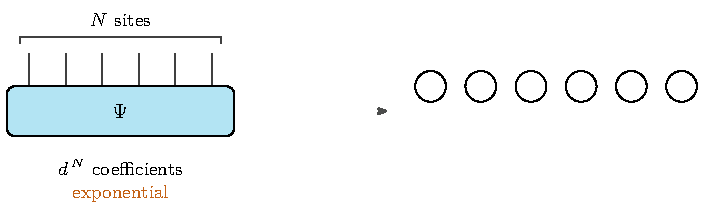
\includegraphics[width=0.86\textwidth]{motivation_tn_a.pdf}}%
    \only<2>{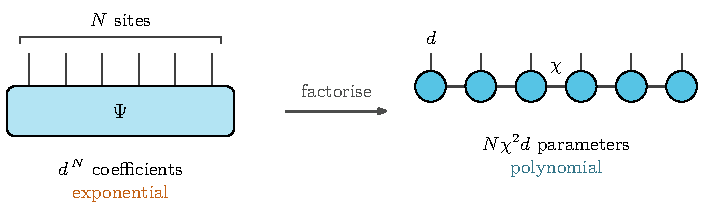
\includegraphics[width=0.86\textwidth]{motivation_tn.pdf}}%
    \only<3>{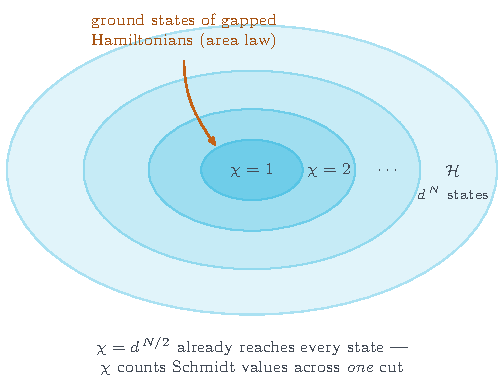
\includegraphics[width=0.48\textwidth]{hilbert_corner.pdf}}
  \end{center}
  % the block must vanish on step 3, or its empty box pushes that caption
  % into the footer
  \only<1-2>{%
      \begin{center}
        \only<1>{$\displaystyle \ket{\Psi} = \sum_{i_1 \dots i_N}
              \hlb{accent}{$\Psi_{i_1 i_2 \cdots i_N}$}\;
              \ket{i_1 i_2 \cdots i_N}$}%
        \only<2>{$\displaystyle \hlb{accent}{$\Psi_{i_1 i_2 \cdots i_N}$}
              \;=\; \sum_{\alpha_1 \dots \alpha_{N-1}}
              A^{i_1}_{\alpha_1}\,A^{i_2}_{\alpha_1\alpha_2}\cdots
              A^{i_N}_{\alpha_{N-1}}$}%
      \end{center}}
  \begin{center}\small\color{ink!75}
    \only<1>{the \textbf{many-body problem}: a state is a list of $d^N$ numbers}%
    \only<2>{a \textbf{matrix product state (MPS)}: \ $\chi$ $=$ the
        entanglement it can carry $=$ the memory it costs}%
    \only<3>{a small $\chi$ already describes states with low entanglement\\
        and fast-decaying correlations --- the \textbf{area law}}%
  \end{center}
  \vfill
\end{frame}

% ============================================================================
% READING A TENSOR NETWORK — the diagram grammar, and why 2D is hard
% ============================================================================
\begin{frame}{Reading a Tensor Network}
  \vfill
  \begin{center}
    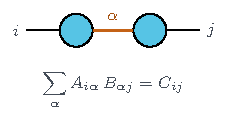
\includegraphics[width=0.28\textwidth]{tn_contract.pdf}\\[0.4ex]
    {\small joining two legs $=$ summing over that index $=$
      a \textbf{contraction}}
  \end{center}
  \vfill
  \begin{center}
    \makebox[0.65\textwidth][c]{%
      \visible<2->{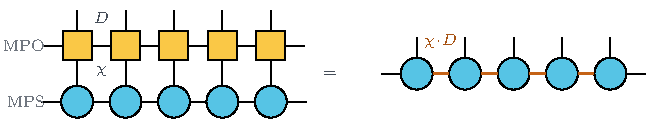
\includegraphics[width=0.64\textwidth]{tn_apply.pdf}}}%
    \makebox[0.35\textwidth][c]{%
      \visible<3->{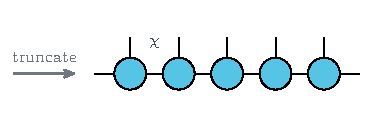
\includegraphics[width=0.358\textwidth]{tn_trunc.pdf}}}
  \end{center}
  \vspace{-0.1em}
  \begin{center}\small
    \makebox[0.65\textwidth][c]{%
      \visible<2->{an \textbf{MPO}: an operator in the same language}}%
    \makebox[0.35\textwidth][c]{%
      \visible<3->{keep the largest Schmidt values}}
  \end{center}
  \vfill
\end{frame}

% ============================================================================
% MOTIVATION II — the entanglement barrier
% ============================================================================
\begin{frame}{Dynamics: the Entanglement Barrier}
  \begin{columns}[c]
    \begin{column}{0.44\textwidth}
      \begin{center}\small
        dynamics runs into a different problem:
      \end{center}
      \vspace{-0.2em}
      \begin{center}\small
        $\chi \;\xrightarrow{\ \text{apply MPO}\ }\; D\chi
          \;\xrightarrow{\ \text{truncate}\ }\; \chi$
      \end{center}
      \vspace{0.5em}
      \begin{center}
        {\footnotesize\color{ink!70} after a quench:}\\[0.3ex]
        $S_x(t)\sim t \;\;\Longrightarrow\;\; \chi\sim e^{ct}$
      \end{center}
      \vspace{0.3em}
      \onslide<2->{\idea{this work: time evolution\\ that avoids the barrier,\\
            for critical quenches in 1D}}
    \end{column}
    \begin{column}{0.54\textwidth}
      \centering
      % the band marks where the run has hit the bond-dimension cap and the
      % answer stops being the physics. Coordinates are fractions of the
      % image, so they follow the figure if it is ever resized.
      \begin{tikzpicture}
        \node[inner sep=0,anchor=south west] (bimg) at (0,0)
        {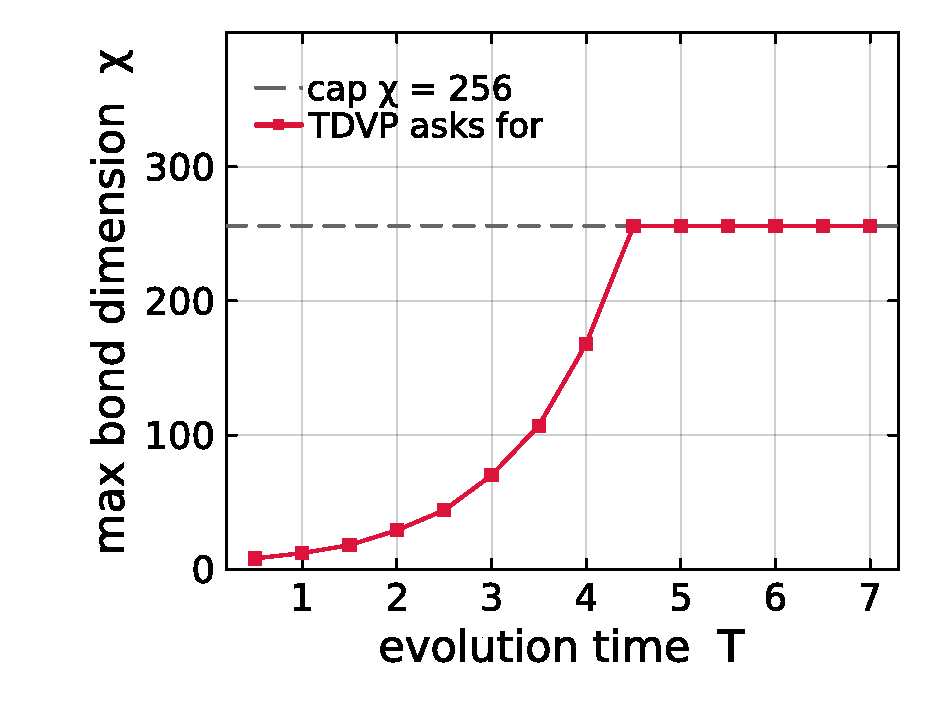
\includegraphics[width=\textwidth]{entanglement_barrier.pdf}};
        % band spans from where the run first hits the cap (T = 4.5) to the
        % right edge of the axes; fractions measured off the figure itself.
        \begin{scope}[x={(bimg.south east)},y={(bimg.north west)}]
          \fill[warn,opacity=0.12] (0.680,0.218) rectangle (0.965,0.957);
        \end{scope}
      \end{tikzpicture}
    \end{column}
  \end{columns}
\end{frame}

% ============================================================================
% WHAT WE WANT OUT OF IT — the universal data, before any CFT
% ============================================================================
\begin{frame}{What We Are Trying to Extract}
  \vfill
  \begin{center}\large
    at a critical point the microscopic details stop mattering, and the model\\
    is described by a set of \textbf{universal numbers}
  \end{center}
  \vspace{0.6em}
  \begin{center}
    \begin{minipage}{0.44\textwidth}\centering
      \tint{accent}{\parbox{0.82\textwidth}{\centering
          \large $c = \tfrac12$\\[0.4ex]
          {\footnotesize\color{ink!70} the \textbf{central charge}}}}
    \end{minipage}%
    \begin{minipage}{0.52\textwidth}\centering
      \tint{hl}{\parbox{0.86\textwidth}{\centering
          \large $x_\alpha \in \big\{\tfrac12,\ \tfrac32,\ 2,\ \tfrac52,\ \dots\big\}$\\[0.4ex]
          {\footnotesize\color{ink!70} the \textbf{boundary operators'}
            dimensions}}}
    \end{minipage}
  \end{center}
  \vspace{0.4em}
  \begin{center}\small\color{ink!75}
    the numbers the \textbf{conformal field theory (CFT)} of the Ising class
    predicts
  \end{center}
  \vfill
  \idea{read them off a real-time dynamical object at the critical point}
  \vspace{0.2em}
  \begin{center}
    \tint{jwnnn}{already done for \textbf{exactly solvable} models
      --- we target the \textbf{non-integrable} ones}\\[0.4ex]
    \src{Carignano \& Tagliacozzo, \emph{Quantum} (2025)}
  \end{center}
  \vfill
\end{frame}

% ============================================================================
% OUTLINE — the arc, then the roadmap. Two steps, one frame.
% ============================================================================
\slidesection{roadmap}
\begin{frame}{Outline}
  \vfill
  \begin{center}
    \textbf{transverse contraction} reaches long evolution times\\[0.35ex]
    $\longrightarrow$ time-evolve a \textbf{non-integrable} chain and compute
    the Loschmidt echo\\[0.35ex]
    $\longrightarrow$ extract its \textbf{universal data} from the simulations\\[0.35ex]
    $\longrightarrow$ compare with the \textbf{CFT predictions}
  \end{center}
  \vfill
  \onslide<2->{%
      {\centering\small
        \setlength{\tabcolsep}{7pt}\renewcommand{\arraystretch}{1.28}%
        \begin{tabular}{@{}r l c@{}}
          1. & the Loschmidt echo and the CFT mapping     &                          \\
          2. & transverse contraction                     &                          \\
          3. & the model and its equilibrium properties   & \hlt{accent}{$\bigstar$} \\
          4. & a translation-invariant evolution operator & \hlt{accent}{$\bigstar$} \\
          5. & power iterations: the dominant pair        &                          \\
          6. & the block power method: the tower          & \hlt{accent}{$\bigstar$} \\
          7. & results                                    &                          \\
        \end{tabular}\par}}
  \vfill
\end{frame}

% ============================================================================
% THE LOSCHMIDT ECHO — one visual identity
% ============================================================================
\slidesection{1 $\cdot$ the echo}
\begin{frame}{The Loschmidt Echo}
  \vfill
  \begin{center}
    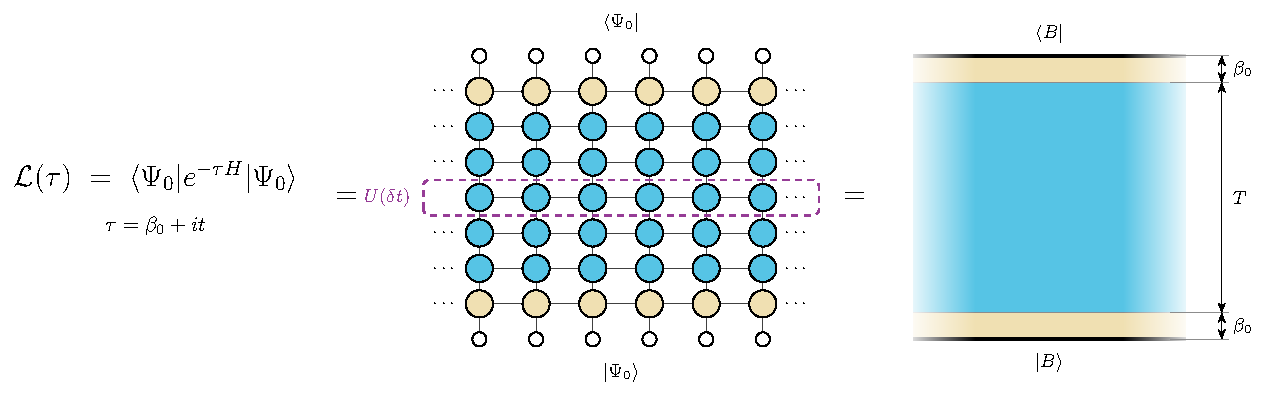
\includegraphics[width=0.97\textwidth]{echo_identity.pdf}
  \end{center}
  \vfill
  \begin{center}
    $e^{-iHT}
      \;\xrightarrow[\;\text{\footnotesize rotation } T\,\to\,-i\tau\;]{}\;
      e^{-\tau H}$
    \quad\raisebox{0.1ex}{\footnotesize\color{ink!70}%
      Euclidean partition function --- where the CFT applies}
  \end{center}
  \vspace{-0.4em}
  \begin{center}
    \small strip width $\,\beta = v\,(2\beta_0 + iT)$, growing with time
  \end{center}
  \vspace{-0.2em}
  \begin{center}\src{Carignano \& Tagliacozzo, \emph{Quantum} (2025)}\end{center}
  \vfill
\end{frame}

% ============================================================================
% TRANSVERSE ROTATION
% ============================================================================
\slidesection{2 $\cdot$ transverse contraction}
\begin{frame}{The Transverse Rotation}
  \begin{columns}[c]
    \begin{column}{0.46\textwidth}
      \centering
      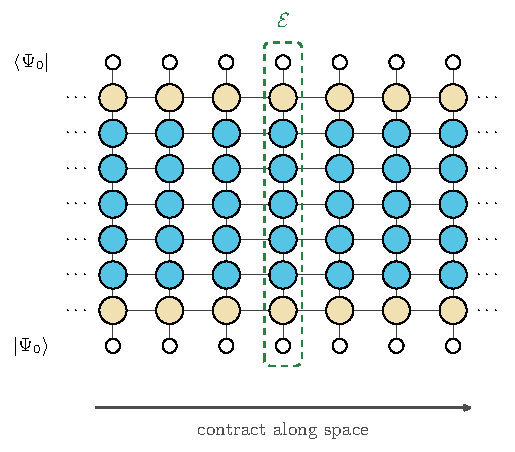
\includegraphics[width=0.88\textwidth]{rotation_network.pdf}
    \end{column}
    \begin{column}{0.52\textwidth}
      \centering
      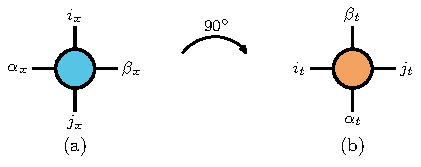
\includegraphics[width=0.94\textwidth]{rotation.pdf}\\[1.2ex]
      {\small virtual space $\to$ physical \emph{time}\\
        physical space $\to$ virtual direction}
      \idea{translation invariance $\Rightarrow$ every column is\\ the same
        operator: the transfer matrix $\E$}
      \begin{center}\src{Ba\~nuls et al.\ (2009) $\cdot$ code:
          \texttt{ITransverse.jl}, Carignano (2026)}\end{center}
    \end{column}
  \end{columns}
\end{frame}

% ============================================================================
% EIGENPROBLEM
% ============================================================================
\begin{frame}{Dynamics as an Eigenproblem}
  \begin{columns}[c]
    \begin{column}{0.42\textwidth}
      \[
        \Lech(T) \;=\; \bra{b_L}\,\E^{\,N}\ket{b_R}
        \;=\; \sum_i c_i\,\mu_i^{\,N}
      \]
      \vspace{-1.7em}
      \[
        =\; \hlb{accent}{$c_0\,\mu_0^{\,N}$}
        \underbrace{\Big[\,1+\sum_{i\ge1}\tfrac{c_i}{c_0}
            \big(\tfrac{\mu_i}{\mu_0}\big)^{\!N}\Big]}_{\textstyle\to\,1}
      \]
      \vspace{0.9em}
      \begin{center}\footnotesize\color{ink!70}
        $\E\ket{r_i}=\mu_i\ket{r_i}$, \quad $\bra{\ell_i}\E=\mu_i\bra{\ell_i}$\\[0.5ex]
        $c_i=\braket{b_L}{r_i}\braket{\ell_i}{b_R}$
      \end{center}
      \vspace{0.9em}
      \onslide<2->{%
          \idea{$\E\E^\dagger \neq \E^\dagger\E$: everything reduces\\
            to the dominant pair and to the\\
            spectrum of the non-Hermitian $\E$}}
    \end{column}
    \begin{column}{0.56\textwidth}
      \centering
      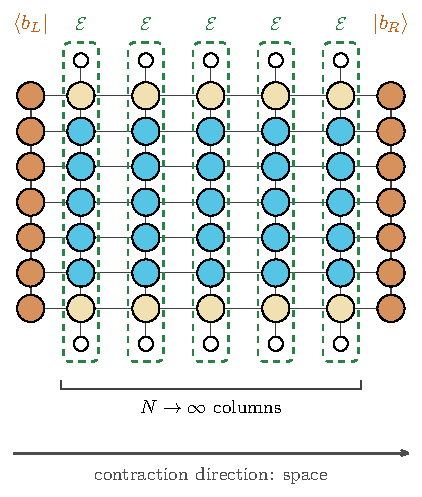
\includegraphics[width=\textwidth,height=0.64\textheight,keepaspectratio]{eigenproblem.pdf}\\[0.6ex]
      \onslide<2->{\footnotesize $b_L$, $b_R$: random seeds --- repeated
          application \emph{projects} them onto the dominant pair,\\
          $\bra{b_L}\E^{N}\!\to\bra{L}$, \ $\E^{N}\ket{b_R}\!\to\ket{R}$}
    \end{column}
  \end{columns}
\end{frame}

% ============================================================================
% WHAT A CFT GIVES US — the vocabulary the predictions are written in
% ============================================================================
\begin{frame}{What a CFT Gives Us}
  \vfill
  \begin{center}
    at a critical point the continuum theory is a\\
    \textbf{conformal field theory (CFT)}\\[0.5ex]
    {\color{accent}$\downarrow$}\ \ so many symmetries that:
  \end{center}
  \vspace{-0.2em}
  \begin{center}\small
    \tint{accent}{\parbox{0.40\textwidth}{\centering
        the whole model is fixed by\\ \textbf{one number}: the central charge $c$}}%
    \quad
    \tint{hl}{\parbox{0.40\textwidth}{\centering
        each operator is fixed by\\ \textbf{one number}: its dimension $x$}}
  \end{center}
  \vfill
  \onslide<2->{%
      \begin{columns}[c]
        \begin{column}{0.30\textwidth}
          {\small map the plane to a \textbf{strip with edges} and some of the
            operators go missing\par}
          \vspace{0.8em}
          {\scriptsize\color{ink!60} each dimension fixes how fast that
            operator's correlations die at the edge\par}
        \end{column}
        \begin{column}{0.68\textwidth}
          \centering
          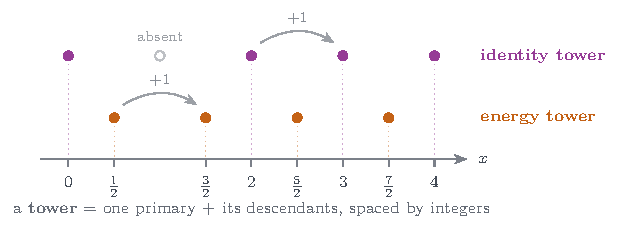
\includegraphics[width=\textwidth]{tower_ladder.pdf}
        \end{column}
      \end{columns}}
  \vfill
\end{frame}

% ============================================================================
% PREDICTIONS I — the spectrum of E
% ============================================================================
\begin{frame}{CFT Predictions I --- the Leading Eigenvalue}
  \vspace{-0.3em}
  \begin{center}\small\color{ink!70}
    after the Wick rotation: a CFT on a strip of width
    $\beta = v\,(2\beta_0 + iT)$
  \end{center}
  \vspace{-0.4em}
  \[
    \E = e^{-\hat H}\;\;(a=1),\qquad
    \hat H = \frac{\pi}{\beta}\Big(\hlt{accent}{L_0} - \frac{c}{24}\Big)
    \qquad\Longrightarrow\qquad
    \mu_i = \exp\Big[-\frac{\pi}{\beta}\Big(\hlt{accent}{x_i}
      - \frac{c}{24}\Big)\Big]
  \]
  \vspace{-0.7em}
  \begin{center}\footnotesize\color{ink!70}
    $\E$ steps one spacing \emph{along} the strip $\Rightarrow$ a weight,
    not a phase\\
    $L_0$: generator of scalings, eigenvalues $x_i$ \quad$\cdot$\quad
    $-c/24$: the Casimir shift
  \end{center}
  \vfill
  \onslide<2->{%
      1.\ emergent dual unitarity --- the moduli lock:
      \[
        \frac{|\mu_i|}{|\mu_0|} = 1 - \frac{b_i}{T^2}
        \;\longrightarrow\; 1
      \]}
  \vfill
  \onslide<3->{%
      2.\ the dominant phase --- the expression we fit:
      \[
        \frac{\operatorname{Im}\lambda_0}{T}
        = a_0 + \frac{B}{T} + \frac{C}{T^{2}},
        \qquad B = -\pi \ \text{(branch, fixed)}
        \qquad\Longrightarrow\qquad
        c = \frac{24\,v\,|C|}{\pi}
      \]
      \vspace{-0.7em}
      \begin{center}\footnotesize\color{ink!70}
        $\lambda_0=\log(-\mu_0)$, \ and
        $\operatorname{Im}\log\mu = \arg\mu$ --- the phase
      \end{center}}
  \vfill
\end{frame}

% ============================================================================
% PREDICTIONS II — boundary operator content
% ============================================================================
\begin{frame}{CFT Predictions II --- the Operator Content}
  \begin{columns}[c]
    \begin{column}{0.44\textwidth}
      \[
        \Delta\theta_\alpha \;=\; \arg\mu_\alpha - \arg\mu_0
        \;=\; \frac{\pi\,\hlb{hl}{$v$}\, x_\alpha}{T}
      \]
      \idea{each subleading eigenvalue\\ $\longleftrightarrow$ one boundary
        operator}
      \vspace{0.1em}
      \begin{center}\small
        so for the Ising class we should see\\[0.4ex]
        $\mu_0$, then one eigenvalue per\\[0.2ex]
        $x_\alpha \in \big\{\tfrac12,\ \tfrac32,\ 2,\ \tfrac52,\ \dots\big\}$
      \end{center}
      \begin{center}\src{Cardy, \emph{Nucl.\ Phys.\ B} (1986)}\end{center}
    \end{column}
    \begin{column}{0.54\textwidth}
      \centering
      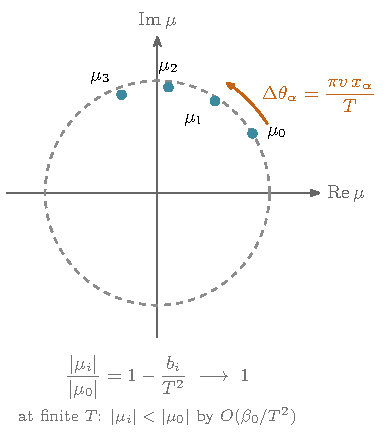
\includegraphics[width=0.85\textwidth]{spectrum_sketch.pdf}
    \end{column}
  \end{columns}
\end{frame}

% ============================================================================
% RTM + PREDICTIONS II
% ============================================================================
\begin{frame}{Temporal Entropies from the Cut: the RTM}
  \vfill
  \begin{center}\large\color{ink!85}
    cost of the contraction $=$ entanglement across a cut in \textbf{time}
  \end{center}
  \vfill
  \visible<2->{%
      \begin{center}
        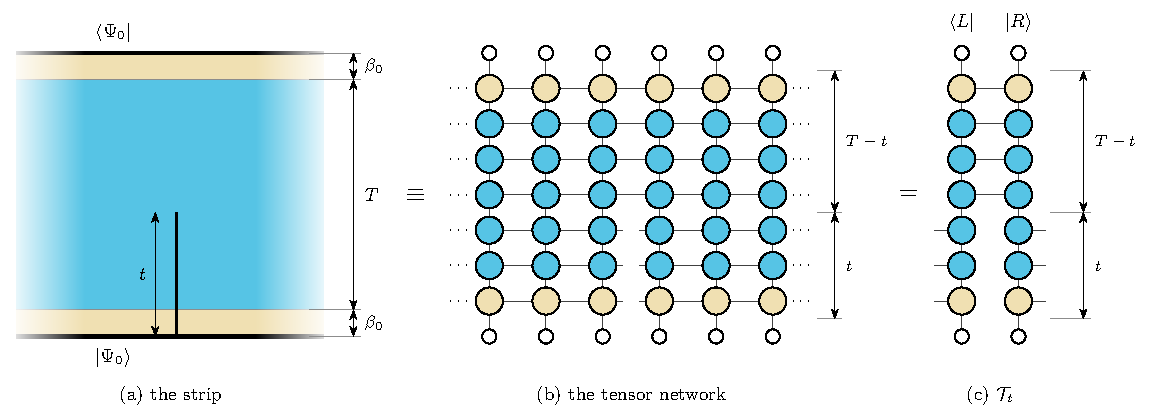
\includegraphics[width=0.72\textwidth,height=0.50\textheight,keepaspectratio]{rtm_strip.pdf}
      \end{center}}
  \vfill
  \visible<3->{%
      \[
        \mathcal{T}_t \;=\; \frac{\Tr_{>t}\,\ket{R}\bra{L}}{\braket{L}{R}}
        \qquad\qquad
        S_2^{\mathrm{gen}}(t)
        \;=\; -\ln \Tr\!\left(\mathcal{T}_t^{\,2}\right)
      \]}
  \vfill
\end{frame}

% ============================================================================
% PREDICTIONS III — the temporal entropy
% ============================================================================
\begin{frame}{CFT Predictions III --- the Temporal Entropy}
  \vfill
  \[
    \operatorname{Re} S_2^{\mathrm{gen}}(t)
    \;=\; s_0 + \frac{c}{8}\,
    \log\!\Big[\frac{2T}{\pi}\sin\frac{\pi t}{T}\Big]
    \qquad \text{(chord dome)}
  \]
  \vfill
  \[
    \operatorname{Im} S_2^{\mathrm{gen}}(t)
    \;=\; \frac{\pi c}{16}
    \qquad \text{(constant plateau)}
  \]
  \vfill
  \onslide<2->{\idea{logarithmic in $T$ $\;\Rightarrow\;$ polynomial resources}}
  \vfill
  \begin{center}\src{Calabrese \& Cardy, \emph{J.\ Stat.\ Mech.} (2004)}\end{center}
\end{frame}

% ============================================================================
% THE MODEL + its equilibrium central charge
% ============================================================================
\slidesection{3 $\cdot$ the model}
\begin{frame}{The ANNNI-type Chain Stays in the Ising Class}
  \vspace{-0.2em}
  \[
    H = -\sum_i\Big[
    \underbrace{\hlt{jwnn}{\sigma^z_i\sigma^z_{i+1} + \lambda\,\sigma^x_i}}
    _{\text{\scriptsize\color{jwnn}transverse-field Ising}}
    + \underbrace{p\big(\hlt{jwnnn}{\sigma^z_i\sigma^z_{i+2}}
    + \hlt{jwxx}{\lambda\,\sigma^x_i\sigma^x_{i+1}}\big)}
    _{\text{\scriptsize\color{ink!55}new with $p$}}
    \Big],
    \quad \lambda = 1
  \]
  \vspace{-0.6em}
  \begin{center}
    {\scriptsize\color{ink!60} after a Jordan--Wigner transformation:}\\[0.25ex]
    {\small
      \tint{jwnn}{$p=0$: \textbf{free} fermions --- solvable exactly}\quad
      \tint{jwnnn}{$p>0$: \textbf{interacting} fermions}\par}
  \end{center}
  \pause
  \vspace{-0.5em}
  \begin{columns}[c]
    \begin{column}{0.40\textwidth}
      \centering
      but is it still Ising?\\ ask the ground state:
      \[
        S_{\mathrm{vN}}(l,L) = \frac{c}{6}\,
        \underbrace{\log\!\Big[\frac{2L}{\pi}\sin\frac{\pi l}{L}\Big]}_{\textstyle W}
        + k
      \]
      \idea{DMRG, $N=400$\\ $c=0.50$ for every $p$}
    \end{column}
    \begin{column}{0.58\textwidth}
      \centering
      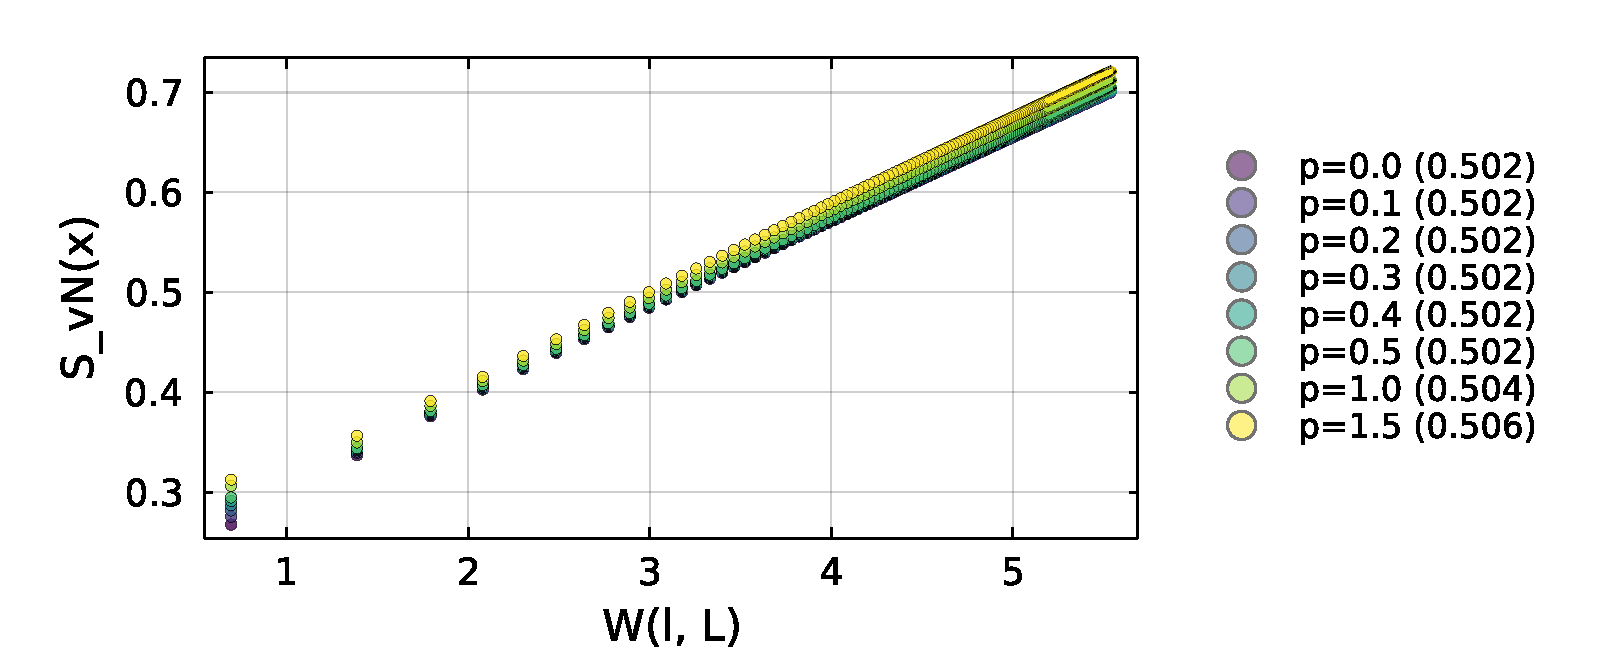
\includegraphics[width=0.94\textwidth]{cft_chord_equilibrium.pdf}
    \end{column}
  \end{columns}
\end{frame}

% ============================================================================
% EQUILIBRIUM VELOCITY
% ============================================================================
\begin{frame}{The Sound Velocity}
  \vspace{-0.8em}
  \hfill{\footnotesize\color{ink!70} $v\,T =$ conformal distance in the strip}
  \vspace{0.3em}
  \begin{columns}[c]
    \begin{column}{0.40\textwidth}
      \small diagonalise small rings of $N$ sites exactly:
      \[
        v(N) = \frac{N}{2\pi}\big[E_1(2\pi/N)-E_1(0)\big]
      \]
      \[
        v(N) = v_\infty + \frac{C}{N^2}
      \]
      \begin{center}\small
        finite-size correction, exponent fixed\\ empirically
        ($v=2$ at $p=0$ as reference)
      \end{center}
      \begin{center}\src{estimator: Alcaraz, \emph{Phys.\ Rev.\ B} (2016)}\end{center}
    \end{column}
    \begin{column}{0.58\textwidth}
      \centering
      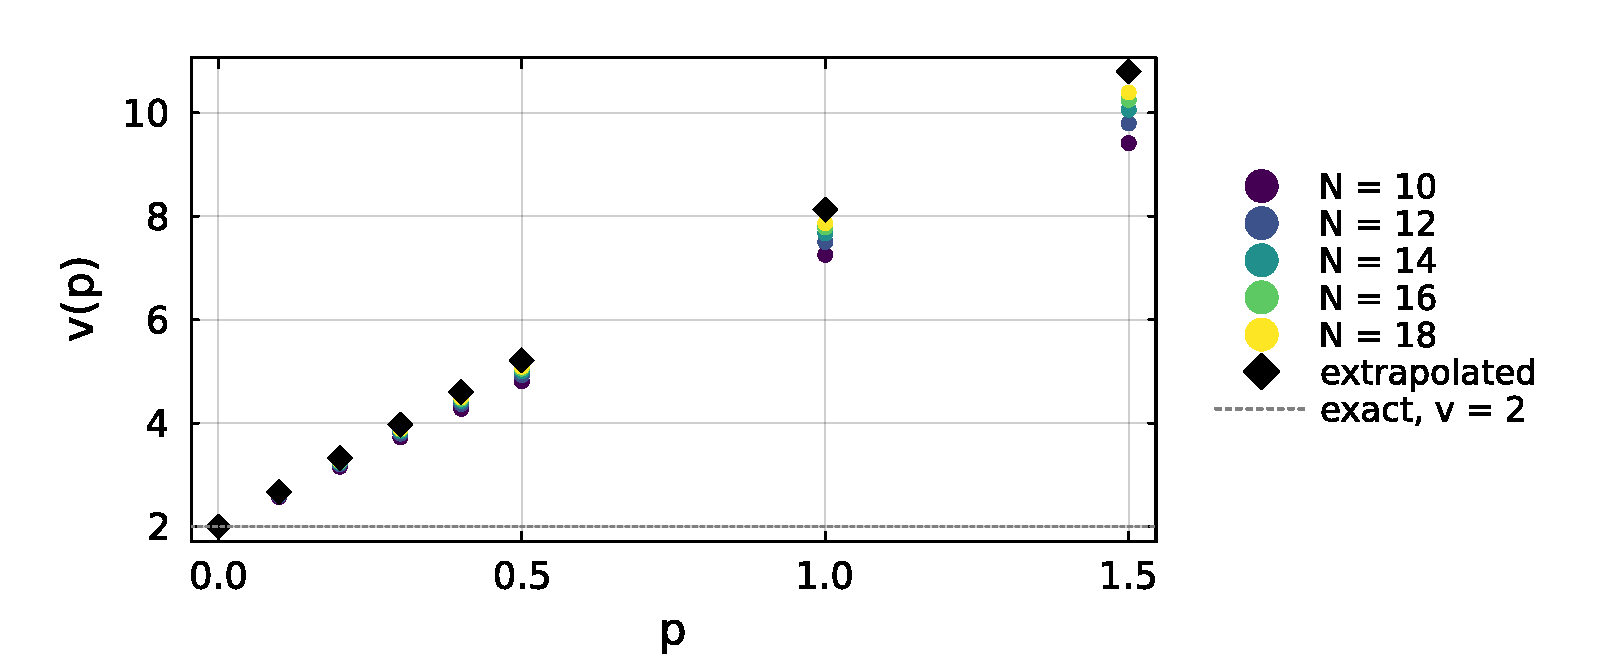
\includegraphics[width=\textwidth]{velocity_vs_p.pdf}
    \end{column}
  \end{columns}
\end{frame}

% ============================================================================
% TRANSLATION-INVARIANT MPO
% ============================================================================
\slidesection{4 $\cdot$ methods}
\begin{frame}{The Time Evolution Operator}
  \begin{columns}[c]
    \begin{column}{0.46\textwidth}
      \centering
      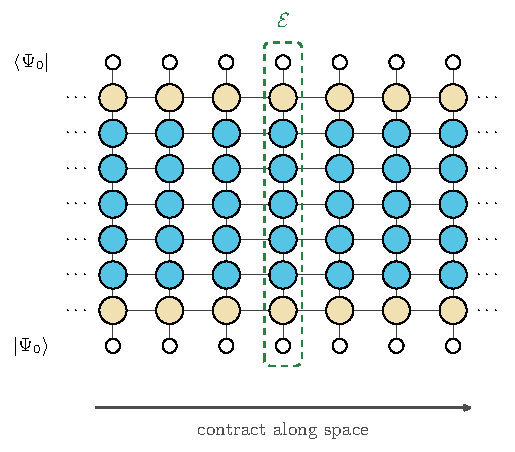
\includegraphics[width=0.9\textwidth]{rotation_network.pdf}
    \end{column}
    \begin{column}{0.52\textwidth}
      \idea{translation invariance $\Rightarrow$\\ $U(\delta t)$ built from
        \textbf{one repeated bulk tensor} $W$}
      \vspace{1.0em}
      \idea{second order in $\delta t$}
    \end{column}
  \end{columns}
\end{frame}

% ============================================================================
% FSM
% ============================================================================
\begin{frame}{The Hamiltonian as a Finite State Machine}
  \vspace{-0.3em}
  {\centering\footnotesize
    $H = -\sum_i\big[\hlt{jwnn}{\sigma^z_i\sigma^z_{i+1} + \lambda\sigma^x_i}
        + p(\hlt{jwnnn}{\sigma^z_i\sigma^z_{i+2}}
        + \hlt{jwxx}{\lambda\sigma^x_i\sigma^x_{i+1}})\big]$\par}
  \vspace{0.2em}
  \onslide<2->{%
      \begin{columns}[c]
        \begin{column}{0.46\textwidth}
          \footnotesize
          \[
            W_H =
            \begin{pmatrix}
              \mathbb{1} & C & D          \\
              0          & A & B          \\
              0          & 0 & \mathbb{1}
            \end{pmatrix}
          \]
          \vspace{-0.7em}
          \begin{center}
            \resizebox{0.90\linewidth}{!}{$\displaystyle
                =\;
                \begin{pmatrix}
                  \mathbb{1} & \hlt{jwnn}{-\sigma^z}     & \hlt{jwxx}{-p\lambda\,\sigma^x}
                             & \hlt{jwnnn}{-p\,\sigma^z} & \hlt{jwnn}{-\lambda\,\sigma^x}                             \\
                  0          & 0                         & 0                               & 0 & \hlt{jwnn}{\sigma^z} \\
                  0          & 0                         & 0                               & 0 & \hlt{jwxx}{\sigma^x} \\
                  0          & \hlt{jwnnn}{\mathbb{1}}   & 0                               & 0 & 0                    \\
                  0          & 0                         & 0                               & 0 & \mathbb{1}
                \end{pmatrix}$}
          \end{center}
          \vspace{0.2em}
          \begin{center}
            $D_W = 1 + 3 + 1 = 5$\\[0.2ex]
            {\footnotesize\color{ink!70} idle $\cdot$ three memory channels
              $\cdot$ done}
          \end{center}
        \end{column}
        \begin{column}{0.52\textwidth}
          \centering
          \onslide<3->{%
              
\includegraphics[width=\textwidth]{fsm.pdf}\\[0.4ex]
              {\footnotesize\color{ink!70} directional machine $\Rightarrow$
                $\E$ \textbf{non-normal}}}
        \end{column}
      \end{columns}}
\end{frame}

% ============================================================================
% VD2
% ============================================================================
\begin{frame}{Exponentiating the MPO: the VD2 Construction}
  \vfill
  \begin{center}
    $\displaystyle
      e^{\tau H} = \mathbb{1} + \tau\sum_x H_x
      + \frac{\tau^2}{2}
      \underbrace{\hlt{hl}{\sum_{x,y} H_x H_y}}
      _{\text{\footnotesize\color{hl!85!black}including the
          \textbf{overlapping} pairs}}
      + \dots$
    \\[2.0ex]
    {\footnotesize\color{ink!70} $\tau = -i\,\delta t$}
  \end{center}
  \vfill
  \onslide<2->{%
      \idea{keeping the overlapping pairs is what makes it second order}}
  \vfill
  \onslide<3->{%
      \begin{center}\small
        a modification of the finite-state machine:
        \textbf{two machines with two indices},\\ so two terms can be in flight
        at once
      \end{center}
      \vspace{0.3em}
      \begin{center}
        bond $= 1+\chi_H+\chi_H^2 = 13$ \qquad
        \src{Van Damme et al., \emph{SciPost Phys.} \textbf{17}, 135 (2024)}
      \end{center}}
  \vfill
\end{frame}

% ============================================================================
% ONE TENSOR FROM THE BULK
% ============================================================================
\begin{frame}{One Tensor from the Bulk}
  \begin{center}
    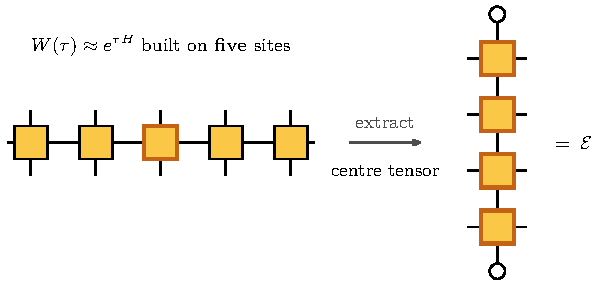
\includegraphics[width=0.88\textwidth,height=0.56\textheight,keepaspectratio]{bulk_extract.pdf}
  \end{center}
  \vfill

\end{frame}

% ============================================================================
% POWER METHOD
% ============================================================================
\begin{frame}{The Power Method: the Dominant Pair}
  \[
    \E\ket{r_i}=\mu_i\ket{r_i},
    \qquad
    \bra{\ell_i}\E=\mu_i\bra{\ell_i},
    \qquad
    \braket{\ell_i}{r_j}=\delta_{ij}
  \]
  \vspace{-0.6em}
  \begin{center}
    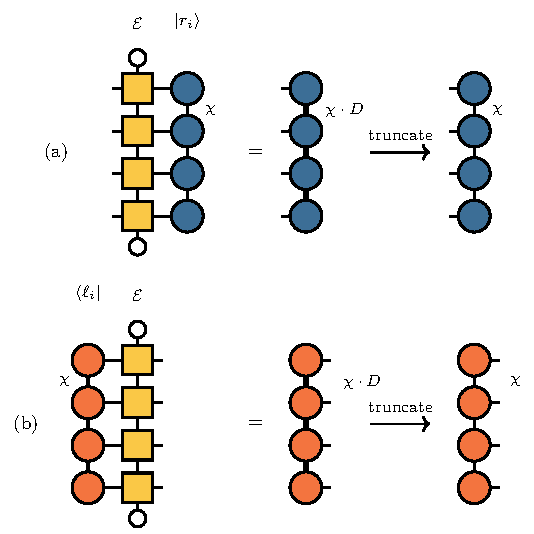
\includegraphics[width=0.88\textwidth]{apply_pair.pdf}
  \end{center}
  \vspace{0.2em}
  \onslide<2->{%
      \begin{columns}[t]
        \begin{column}{0.20\textwidth}
          \raggedleft
          {\large\color{accent!80!black}\textbf{output:}}
        \end{column}
        \begin{column}{0.76\textwidth}
          \raggedright
          1.\ the dominant pair \ $\bra{L}$, $\ket{R}$\\[0.6ex]
          2.\ $\mu_0 \;=\; \dfrac{\bra{L}\,\E\,\ket{R}}{\braket{L}{R}}$
        \end{column}
      \end{columns}
      \vspace{0.4em}
      \hfill{\footnotesize\color{ink!70}
        \textbf{validity}: random complex seeds $\cdot$ independent seeds agree
        $\cdot$ phase continuous in $T$}}
\end{frame}

% ============================================================================
% BLOCK POWER METHOD
% ============================================================================
\begin{frame}{Resolving the Tower: the Block Power Method}
  \vfill
  \begin{center}\large
    the same iteration, on a \textbf{block} of $k$ states per side
  \end{center}
  \vfill
  \[
    \sum_j M_{ij}\, v_j = \theta \sum_j S_{ij}\, v_j,
    \qquad
    S_{ij}=\braket{L_i}{R_j},
    \quad
    M_{ij}=\bra{L_i}\E\ket{R_j}
  \]
  \vspace{-0.6em}
  \begin{center}\footnotesize\color{ink!70}
    a $k\times k$ generalised eigenproblem, projected onto the block
  \end{center}
  \vfill
  \onslide<2->{%
      \idea{$\theta_0,\dots,\theta_{k-1}\;\approx\;\mu_0,\dots,\mu_{k-1}$:
        the $k$ leading eigenvalues,\\ and from their phases the gaps
        $\Delta\theta_\alpha$}}
  \vfill
\end{frame}

% ============================================================================
% RESULTS — opener with the full table
% ============================================================================
\slidesection{5 $\cdot$ results}
\begin{frame}{Results}
  \vfill
  \begin{center}
    {\large the four predictions, measured at every coupling}
  \end{center}
  \vfill
  \fullresults
  \vfill
\end{frame}

% ============================================================================
% RESULTS — entropy route at p = 0
% ============================================================================
\begin{frame}{Results I --- the Entropy Route at $p=0$}
  \vspace{-0.2em}
  \begin{center}\footnotesize\color{ink!70}
    \makebox[0.279\textwidth][c]{\begin{tabular}{@{}c@{}}
        $\operatorname{Re}S_2 = s_0 + \tfrac{c}{8}\,W$ \\[-0.2ex] the dome
      \end{tabular}}%
    \makebox[0.279\textwidth][c]{\begin{tabular}{@{}c@{}}
        $\operatorname{Im}S_2 = \tfrac{\pi c}{16}$ \\[-0.2ex] the plateau
      \end{tabular}}
  \end{center}
  \vspace{-0.4em}
  \begin{center}
    
\includegraphics[width=0.60\textwidth]{res_domes_p0.pdf}
  \end{center}
  \vspace{0.2em}
  \begin{columns}[c]
    \begin{column}{0.55\textwidth}
      \small finite-$T$ correction and extrapolation:
      \vspace{-0.6em}
      \[
        \mathrm{plateau}(T) = a + b\,T^{-1/2}
        \;\Rightarrow\; c = \frac{16\,a}{\pi}
      \]
      \vspace{-1.0em}
      \begin{center}\footnotesize\color{accent!80!black}
        the error bar is the seed-to-seed spread
      \end{center}
    \end{column}
    \begin{column}{0.40\textwidth}
      {\centering\small
        \setlength{\tabcolsep}{5pt}\renewcommand{\arraystretch}{1.1}%
        \tint{routeV}{%
          \begin{tabular}{@{}ccc@{}}
            \toprule
            $p$ & window         & $c$ (entropy) \\
            \midrule
            $0$ & $4\le T\le 22$ & $0.49\pm0.01$ \\
            \bottomrule
          \end{tabular}}\par}
    \end{column}
  \end{columns}
\end{frame}

% ============================================================================
% RESULTS — entropy route, the other couplings
% ============================================================================
\begin{frame}{Results I --- the Entropy Route at Every Coupling}
  \begin{center}
    \domecell{routeV}{res_domes_p0.pdf}{0.49\pm0.01}{$4\le T\le 22$}{$8$--$44$}\hfill
    \domecell{routeV}{res_domes_p01.pdf}{0.50\pm0.04}{$4\le T\le 13$}{$11$--$35$}\\[0.8ex]
    \domecell{hl}{res_domes_p03.pdf}{0.53\pm0.04}{$2\le T\le 9$}{$8$--$36$}\hfill
    \domecell{hl}{res_domes_p05.pdf}{0.58\pm0.04}{$2\le T\le 5$}{$10$--$26$}
  \end{center}
\end{frame}

% ============================================================================
% RESULTS — emergent dual unitarity
% ============================================================================
\begin{frame}{Results II --- Emergent Dual Unitarity}
  \begin{columns}[c]
    \begin{column}{0.4\textwidth}
      \idea{$|\mu_0|$ constant\\ while the phase winds}
      \begin{center}
        $\dfrac{|\mu_i|}{|\mu_0|} = 1 - \dfrac{b_i}{T^2} \to 1$
      \end{center}
      \begin{center}\src{Carignano \& Tagliacozzo (2025)}\end{center}
    \end{column}
    \begin{column}{0.58\textwidth}
      \centering
      \animategraphics[autoplay,loop,poster=last,width=0.95\textwidth]%
      {12.5}{gif_frames/circ_}{0000}{0160}\\[-0.2ex]
      {\scriptsize\color{ink!70} animated in Acrobat; static frame elsewhere}
    \end{column}
  \end{columns}
\end{frame}

% ============================================================================
% RESULTS — central charge from the phase
% ============================================================================
\begin{frame}{Results III --- the Central Charge from the Phase}
  \begin{columns}[c]
    \begin{column}{0.62\textwidth}
      \centering
      
\includegraphics[width=\textwidth,height=0.70\textheight,keepaspectratio]{res_eq3.pdf}
    \end{column}
    \begin{column}{0.36\textwidth}
      \centering
      \[
        \frac{\operatorname{Im}\lambda_0}{T}
        = a_0 + \frac{B}{T} + \frac{C}{T^{2}}
      \]
      \vspace{-0.5em}
      {\small
        \setlength{\tabcolsep}{4pt}\renewcommand{\arraystretch}{1.15}%
        \begin{tabular}{@{}r@{\ }l@{}}
          $a_0,\,C$ & free              \\
          $B=-\pi$  & fixed (branch)    \\
          $c$       & $=24\,v\,|C|/\pi$ \\
        \end{tabular}\par}
      \medskip
      \spectralminitable
    \end{column}
  \end{columns}
  \vfill
  \onslide<2->{%
      \begin{center}\small
        $\dfrac{\operatorname{Im}\lambda_0}{T}
          = a_0 + \dfrac{B}{T} + \dfrac{C}{T^{2}}
          \;\hlb{warn}{$+\,\dfrac{D}{T^{4}}$}\;+\dots$
        \qquad{\footnotesize\color{warn!85!black}
          dropped $\Rightarrow$ bias in $c$}
      \end{center}}
\end{frame}

% ============================================================================
% RESULTS — the boundary tower
% ============================================================================
\begin{frame}{Results IV --- the Conformal Boundary Tower}
  \begin{center}
    Ising class, free boundaries: \
    $x_\alpha \in \big\{\hlt{hl}{\tfrac12},\ \hlt{hl}{\tfrac32},\ \hlt{jwnnn}{2},\
      \hlt{hl}{\tfrac52},\ \hlt{jwnnn}{3},\ \hlt{hl}{\tfrac72},\
      \hlt{jwnnn}{4}\big\}$\\[0.3ex]
    {\footnotesize \hlt{jwnnn}{\textbf{identity tower}} $\;+\;$
      \hlt{hl}{\textbf{energy tower}}}
  \end{center}
  \begin{columns}[c]
    \begin{column}{0.62\textwidth}
      \centering
      
\includegraphics[width=\textwidth,height=0.66\textheight,keepaspectratio]{res_tower.pdf}
    \end{column}
    \begin{column}{0.36\textwidth}
      \[
        \Delta\theta_\alpha = \arg\mu_\alpha - \arg\mu_0
        = \frac{\pi v\, x_\alpha}{T}
      \]
      \vspace{-0.9em}
      \begin{center}\footnotesize\color{ink!70}
        block iteration with $k=8$:\\ the eight leading eigenvalues
      \end{center}
      \vspace{-0.2em}
      \towerminitable
    \end{column}
  \end{columns}
\end{frame}

% ============================================================================
% CONCLUSIONS
% ============================================================================
\slidesection{conclusions}
\begin{frame}{Summary of Results}
  \vfill
  \begin{center}\large
    the conformal signatures in the Loschmidt echo\\[0.2ex]
    \textbf{survive when integrability is broken}
  \end{center}
  \vfill
  \fullresults
  \vspace{0.6em}
  \begin{center}\small
    $c$ from \textbf{two dynamical routes} and \textbf{one equilibrium}
    $\;+\;$ the \textbf{boundary content}
  \end{center}
  \vfill
\end{frame}

% ============================================================================
% WHAT I BUILT — the contribution, stated as a contribution
% ============================================================================
\begin{frame}{Conclusions and Outlook}
  \vfill
  {\centering
    \setlength{\tabcolsep}{6pt}\renewcommand{\arraystretch}{1.45}%
    \begin{tabular}{@{}c l l@{}}
      \hlt{accent}{$\bigstar$} & a translation-invariant 2nd-order MPO
                               & {\small\color{ink!70} for the NNN chain}                                \\
      \hlt{accent}{$\bigstar$} & a block power method
                               & {\small\color{ink!70} subleading spectrum of a non-Hermitian $\E$}      \\
      \hlt{accent}{$\bigstar$} & the equilibrium inputs, measured
                               & {\small\color{ink!70} $v_\infty$ by exact diagonalisation, $c$ by DMRG} \\
      \hlt{accent}{$\bigstar$} & the numerical simulations
                               & {\small\color{ink!70} four couplings, local $+$ cluster}                \\
      \hlt{accent}{$\bigstar$} & the fits, windows and error analysis
                               & {\small\color{ink!70} criteria for convergence of iteration methods}    \\
    \end{tabular}\par}
  \vfill
  \onslide<2->{%
      \begin{center}
        \tint{warn}{\parbox[t]{0.42\textwidth}{\centering
            \textbf{open} \\[0.3ex] {\small why do the available $T$ windows\\
              close as $p$ grows?}}}\quad
        \tint{accent}{\parbox[t]{0.42\textwidth}{\centering
            \textbf{next} \\[0.3ex] {\small improve / optimise the block iteration\\
              higher dimensions,\\ other universality classes and models}}}
      \end{center}}
  \vfill
\end{frame}

% ============================================================================
% BACKUP — unnumbered; grouped by question theme
% ============================================================================
% ============================================================================
% THANK YOU
% ============================================================================
\nosection
\begin{frame}{}
  \vfill
  \begin{center}
    {\Huge\color{accent!80!black}\textbf{Thank you for your attention}}\\[1.2ex]
    {\Huge\color{accent!55} :)}
  \end{center}
  \vfill
  \begin{center}
    
\includegraphics[height=1.05cm]{logo_bsc.png}\hspace{1.6cm}
    
\includegraphics[height=1.05cm]{logo_mqst.png}
  \end{center}
  \vspace*{0.4cm}
\end{frame}

\newcounter{finalframe}
\setcounter{finalframe}{\value{framenumber}}
\inappendixtrue

\slidesection{backup $\cdot$ CFT}
\begin{frame}{Backup A1 --- from the Euclidean Strip to Real Time}
  \vfill
  \begin{center}\small\color{ink!75}
    boundary CFT on a Euclidean strip of width $\ell$, cut anchored at the
    edge:
  \end{center}
  \vspace{-0.3em}
  \[
    S_2 = s_0 + \frac{c}{8}\,
    \log\!\Big[\frac{2\ell}{\pi}\sin\frac{\pi x}{\ell}\Big]
  \]
  \vspace{-1.2em}
  \begin{center}\small\color{ink!60}
    $c/8 = (c/12)(1+1/n)$ at $n=2$ --- halved, because an edge-anchored cut
    has one border and not two
  \end{center}
  \vfill
  \begin{center}\small
    continue to real time: \quad $\ell \to i\,vT$, \quad $x \to i\,vt$
  \end{center}
  \vspace{0.2em}
  \begin{center}\small
    the ratio $x/\ell = t/T$ stays real $\Rightarrow$ the sine is
    untouched;\\[0.2ex]
    only the prefactor picks up $\log i = i\pi/2$
  \end{center}
  \vfill
  \[
    \operatorname{Re}S_2 = s_0 + \frac{c}{8}\,W(t,T)
    \quad\text{(dome)}\qquad
    \operatorname{Im}S_2 = \frac{c}{8}\cdot\frac{\pi}{2} = \frac{\pi c}{16}
    \quad\text{(plateau)}
  \]
  \vfill
\end{frame}

\begin{frame}{Backup A2 --- the Spectrum, Derived I: from $T(z)$ to $\mu_i$}
  \vspace{-0.2em}
  \begin{center}\small\color{ink!75}
    $T$: the \textbf{stress tensor} --- the operator that generates conformal
    maps; its modes are the Virasoro generators $L_n$.\\[0.2ex]
    It is not primary: a map adds the inhomogeneous Schwarzian term,
    $\propto c$.
  \end{center}
  \vspace{-0.2em}
  \[
    T(w) = \Big(\frac{dz}{dw}\Big)^2 T(z) + \frac{c}{12}\{z;w\},
    \qquad
    \{z;w\}_{\log} = -\frac12\Big(\frac{\pi}{\beta}\Big)^2
  \]
  \[
    \Longrightarrow\quad
    \hat H = \frac{\pi}{\beta}\Big(L_0 - \frac{c}{24}\Big)
    \qquad\Longrightarrow\qquad
    \mu_i = \exp\Big[-\frac{\pi}{\beta}\Big(x_i - \frac{c}{24}\Big)\Big]
  \]
  \vspace{-0.6em}
  \begin{center}\small\color{ink!75}
    $\hat H$ is not $T$ itself --- it is $T$ \emph{integrated across} the
    strip: the generator of translations \emph{along} it
  \end{center}
  \begin{center}\small
    on the lattice, two non-universal additions --- both the same for
    every level:
  \end{center}
  \[
    E_i \;=\; \underbrace{f\beta}_{\text{bulk}}
    \;+\; \underbrace{f_s}_{\text{boundary}}
    \;+\; \frac{\pi}{\beta}\Big(x_i - \frac{c}{24}\Big),
    \qquad \log\mu_i = -E_i
  \]
  \idea{level-independent terms cancel in every difference ---
    differences isolate $x_i - x_0$}
\end{frame}

\begin{frame}{Backup A3 --- the Spectrum, Derived II: the Expansion We Fit}
  \vspace{-0.4em}
  \[
    \beta = v(2\beta_0 + iT) = i\,vT\Big(1 - \frac{2i\beta_0}{T}\Big)
    \quad\Longrightarrow\quad
    \frac1\beta = \frac{1}{i\,vT}\,\frac{1}{1 - \frac{2i\beta_0}{T}}
    = -\frac{i}{vT}\sum_{k\ge0}\Big(\frac{2i\beta_0}{T}\Big)^{k}
  \]
  \vspace{-0.6em}
  \begin{center}
    \begin{minipage}[c]{0.62\textwidth}\centering
      {\footnotesize\color{ink!70} a geometric series, and it converges:\\
        $2\beta_0/T \le 0.2$ in every run \ ($\beta_0 = 0.2$, $T \ge 2$)}
    \end{minipage}%
    \begin{minipage}[c]{0.30\textwidth}\centering
      {\small$
          \begin{array}{c|cc}
            k & \text{goes to} & \text{order}  \\\hline
            0 & \text{phase}   & 1/T           \\
            1 & \text{modulus} & \beta_0/T^2   \\
            2 & \text{phase}   & \beta_0^2/T^3
          \end{array}$}
    \end{minipage}
  \end{center}
  \[
    \operatorname{Im}\lambda_0 = A\,T + B + \frac{C}{T} + \mathcal{O}(T^{-3}),
    \qquad A=-fv,\quad B=-\pi,\quad C=-\frac{\pi c}{24 v}
  \]
  \begin{center}\small
    no $1/T^2$ term (that order is real $\to$ modulus); $B$ is pure branch
    (free fit: $B/\pi=-1.0000$)\\[0.3ex]
    the fit \textbf{truncates this expansion} $\Rightarrow$ part of the
    systematic on $c$
  \end{center}
  \[
    \frac{|\mu_i|}{|\mu_0|} = 1 - \frac{2\pi\beta_0 (x_i-x_0)}{v\,T^{2}}
    \;\longrightarrow\; 1
    \qquad \text{(the circle)}
  \]
\end{frame}

% ---- backup: the model -----------------------------------------------------------------

\slidesection{backup $\cdot$ the model}
\begin{frame}{Backup B1 --- the Chain in Fermions: Where Integrability Breaks}
  \[
    H = -\sum_i\Big[\hlt{jwnn}{\sigma^z_i\sigma^z_{i+1} + \lambda\,\sigma^x_i}
      + p\big(\hlt{jwnnn}{\sigma^z_i\sigma^z_{i+2}}
      + \hlt{jwxx}{\lambda\,\sigma^x_i\sigma^x_{i+1}}\big)\Big]
  \]
  \begin{center}\small
    Jordan--Wigner: \ $\sigma^x_j = 1-2n_j$, \quad
    $\sigma^z_j = (c_j + c_j^\dagger)\,K_j$, \quad
    $K_j = \prod_{k<j}(1-2n_k)$
  \end{center}
  \[
    \resizebox{0.97\textwidth}{!}{$
  H = -\sum_i\Big[
    \textcolor{jwnn}{\underbrace{(c^\dagger_i - c_i)(c_{i+1}+c^\dagger_{i+1})}_{\text{NN: quadratic}}}
    + \lambda\,\textcolor{jwnn}{\underbrace{(1-2n_i)}_{\text{field: quadratic}}}
    + p\,\textcolor{jwnnn}{\underbrace{(c^\dagger_i - c_i)(1-2n_{i+1})(c_{i+2}+c^\dagger_{i+2})}_{\text{NNN: contains a quartic piece}}}
    + p\lambda\,\textcolor{jwxx}{\underbrace{\big(1-2n_i-2n_{i+1}+4\,n_i n_{i+1}\big)}_{\sigma^x\sigma^x\text{: density--density}}}
    \Big]$}
  \]
  \idea{the $p$-terms carry four-fermion pieces $\Rightarrow$ Wick fails ---
    no free-fermion solution for $p>0$}
\end{frame}

\begin{frame}{Backup B2 --- Equilibrium $c$: Finite-Size Scaling}
  \[
    S_n(L/2) = \frac{c}{12}\Big(1+\frac1n\Big)\ln L + k_n + A_n\,L^{-x/n}
    \qquad \text{(mid-chain cut, $x=1$ fixed)}
  \]
  \begin{center}\small
    $\Longrightarrow\ c = 0.50$ at both couplings
  \end{center}
  \begin{center}
    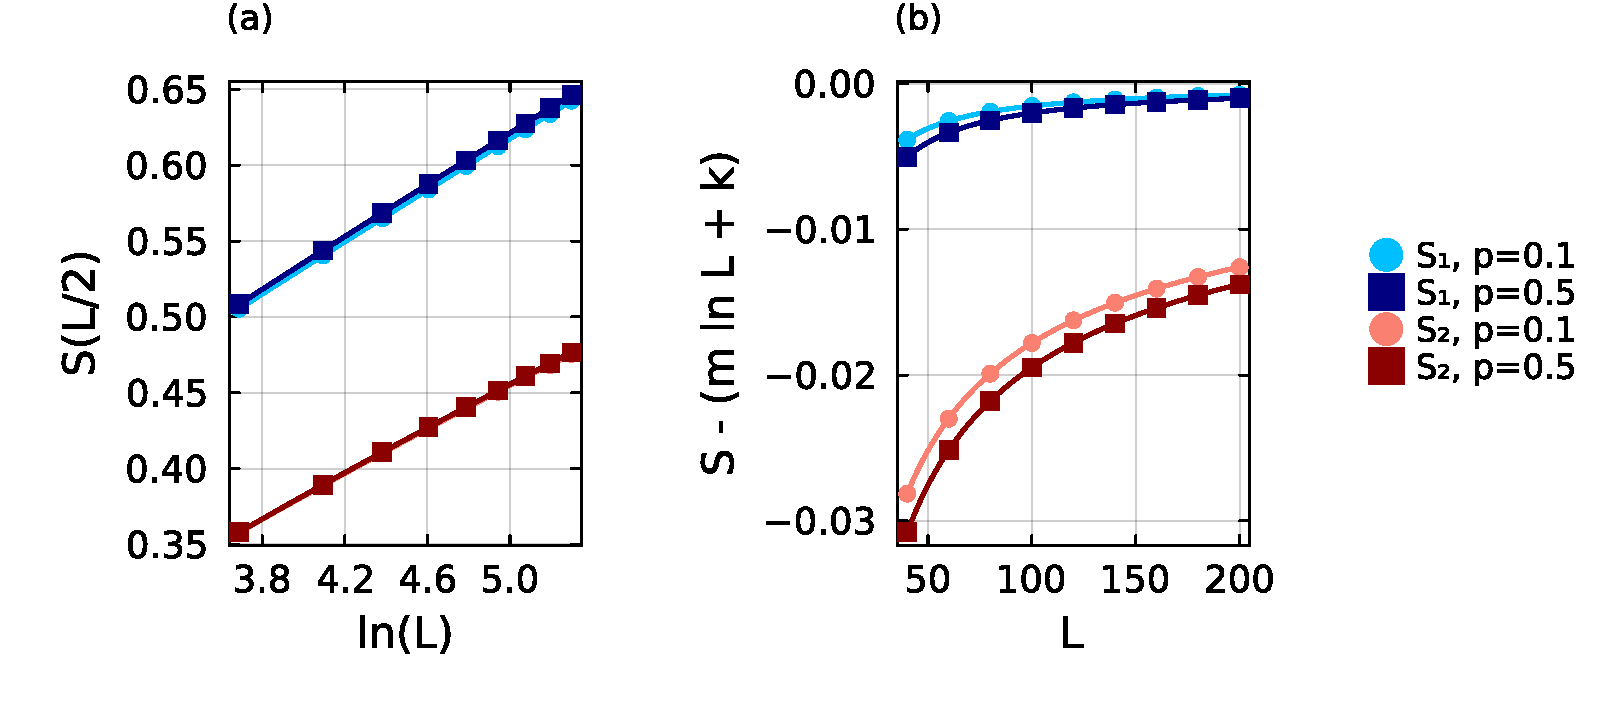
\includegraphics[width=0.86\textwidth,height=0.52\textheight,keepaspectratio]{cft_L.pdf}
  \end{center}
\end{frame}

\begin{frame}{Backup B3 --- Sound Velocity: Extrapolation}
  \[
    v(N) = \frac{N}{2\pi}\big[E_1(2\pi/N)-E_1(0)\big]
    \qquad\qquad
    v(N) = v_\infty +
    \tikz[baseline=(cn.base)]{\node[draw=hl, ellipse, inner sep=2pt,
      line width=0.9pt] (cn) {$\dfrac{C}{N^{2}}$};}
  \]
  \begin{center}
    {\footnotesize\color{hl} empirical term: exponent fixed so the
      extrapolation reproduces $v=2$ exactly at $p=0$}\\[0.2ex]
    {\footnotesize\color{ink!70} the miss there:
      $2{\times}10^{-2}$ ($1/N$) \ $\cdot$ \
      \hlt{hl}{$6{\times}10^{-5}$ ($1/N^{2}$)} \ $\cdot$ \
      $6{\times}10^{-3}$ ($1/N^{3}$)}
  \end{center}
  \begin{center}
    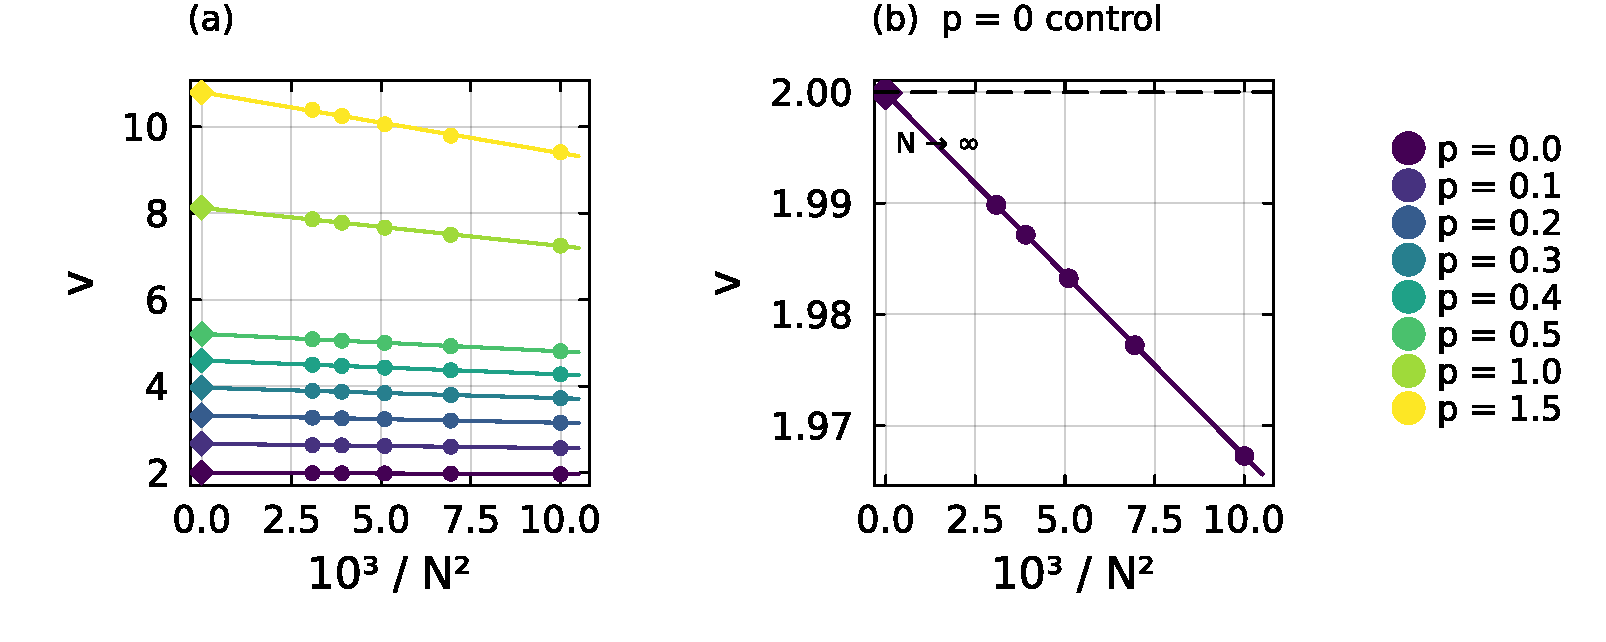
\includegraphics[width=0.82\textwidth,height=0.45\textheight,keepaspectratio]{velocity_extrapolation.pdf}
  \end{center}
\end{frame}

% ---- backup: the MPO -------------------------------------------------------------------

\slidesection{backup $\cdot$ the MPO}
\begin{frame}{Backup C1 --- Schr\"odinger-Picture Benchmark of the MPO}
  \begin{columns}[c]
    \begin{column}{0.46\textwidth}
      the Loschmidt rate we compute:
      \[
        \ell(T) = -\lim_{N\to\infty}\frac{1}{N}\,\log\big|\mathcal{L}(T)\big|
      \]
      \begin{center}\small
        finite chain, $N=40$, $p=0.1$:\\ repeated application of
        $U(\delta t)$ vs a TDVP reference
      \end{center}
      \vspace{0.6em}
      {\scriptsize
        \tint{ink}{\parbox{0.95\textwidth}{\centering
            $W^{\mathrm{I}}$, $W^{\mathrm{II}}$: the same machine, bond $4$
            (VD2: $13$)\\[0.25ex]
            $W^{\mathrm{I}}$: disjoint products only\\[0.25ex]
            $W^{\mathrm{II}}$: $+$ overlaps on one site\\[0.25ex]
            neither: two interactions across the same bond\\[0.25ex]
            $\Rightarrow$ \textbf{first order} in $\delta t$}}\par}
      \vspace{0.2em}
      \begin{center}
        \src{Zaletel et al.\ (2015) $\cdot$ Paeckel et al.\ (2019)}
      \end{center}
    \end{column}
    \begin{column}{0.52\textwidth}
      \centering
      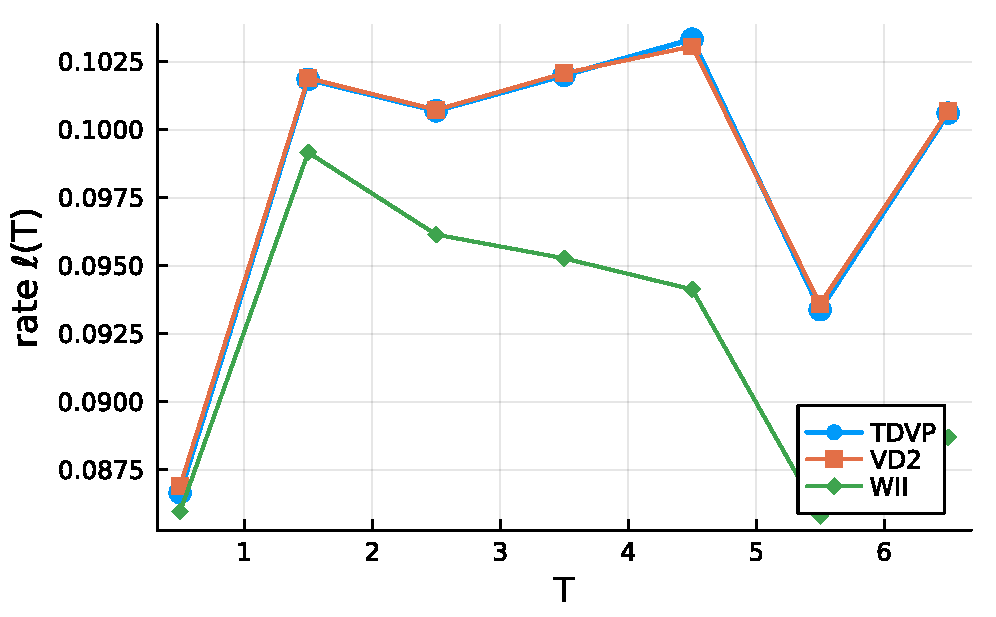
\includegraphics[width=\textwidth]{rate_benchmark.pdf}
    \end{column}
  \end{columns}
\end{frame}

\begin{frame}{Backup C2 --- the Overlap Only VD2 Can Host}
  \vspace{-0.3em}
  \begin{center}\small
    $\displaystyle e^{\tau H} = \mathbb{1} + \tau\sum_x H_x
      + \frac{\tau^2}{2}\,\hlt{hl}{\sum_{x,y} H_x H_y} + \dots$
    \quad{\footnotesize\color{hl!85!black} the overlapping pairs are
      the $\tau^2$ terms at stake}
  \end{center}
  \vspace{-0.2em}
  \begin{center}\small
    the concrete case: $\sigma^z_3\sigma^z_4$ and $\sigma^z_4\sigma^z_5$
    share site $4$
  \end{center}
  \begin{columns}[c]
    \begin{column}{0.42\textwidth}
      \centering
      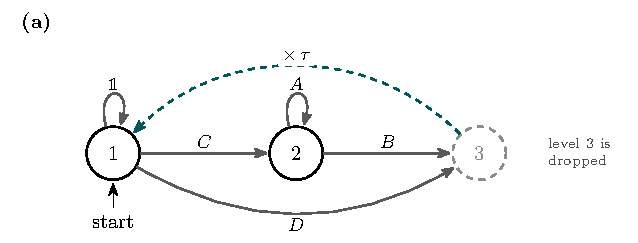
\includegraphics[width=0.90\textwidth]{vd2_panel_a.pdf}\\[0.6ex]
      {\footnotesize site 4 would need $B$ \emph{and} $C$ --- no such
        move exists:\\ the overlap is absent at $\tau^2$}
    \end{column}
    \begin{column}{0.55\textwidth}
      \centering
      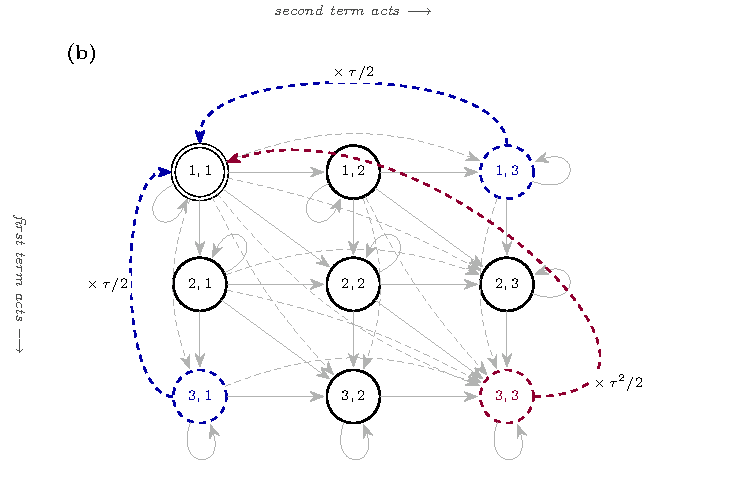
\includegraphics[width=0.96\textwidth,height=0.47\textheight,keepaspectratio]{vd2_panel_b.pdf}\\[0.3ex]
      {\footnotesize
        $(1,1)\xrightarrow{\,C\,}(2,1)
          \xrightarrow{\,BC\,}(3,2)
          \xrightarrow{\,B\,}(3,3)
          \xrightarrow{\text{fold}}\tfrac{\tau^2}{2}$\\[0.2ex]
        (swap the copies $=$ the other ordering)}
    \end{column}
  \end{columns}
\end{frame}

\begin{frame}{Backup C3 --- Norm Drift Under Repeated Application}
  \begin{center}\small
    $\ket{X+}^{\otimes100}$, \ $p=0.1$, \ $\delta t=0.05$, \ cutoff $10^{-12}$
    after every layer
  \end{center}
  \begin{center}
    \setlength{\tabcolsep}{9pt}\renewcommand{\arraystretch}{1.2}
    \begin{tabular}{lccc}
      \toprule
                                      & $W^{\mathrm{I}}$ & $W^{\mathrm{II}}$ & VD2       \\
      \midrule
      virtual bond                    & $4$              & $4$               & $13$      \\
      \midrule
      $\lVert\psi\rVert$, \ 1 layer   & $1.3514$         & $1.1341$          & $0.99995$ \\
      $\lVert\psi\rVert$, \ 8 layers  & $12.6146$        & $3.0181$          & $0.99923$ \\
      $\lVert\psi\rVert$, \ 16 layers & $307.3900$       & $10.8328$         & $0.99751$ \\
      \bottomrule
    \end{tabular}
  \end{center}
  \vfill
  \begin{center}\footnotesize\color{ink!70}
    exact evolution is unitary, so any drift from $1$ is pure construction
    error;\\ reaching $T=10$ at this step takes ${\approx}\,200$ layers
  \end{center}
\end{frame}

\begin{frame}{Backup C4 --- Convergence Orders, Measured}
  \begin{center}\small
    distance to the exactly diagonalised state ($N=12$, $T=1$, $p=0.1$)
  \end{center}
  \begin{center}
    \setlength{\tabcolsep}{5pt}\renewcommand{\arraystretch}{1.0}\small
    \begin{tabular}{lcccccc}
      \toprule
                 & \multicolumn{2}{c}{$W^{\mathrm{I}}$}
                 & \multicolumn{2}{c}{$W^{\mathrm{II}}$}
                 & \multicolumn{2}{c}{VD2}                                                                                          \\[-0.2ex]
      $\delta t$ & error                                 & order  & error                 & order  & error                 & order  \\
      \midrule
      $0.2$      & $2.01{\times}10^{1}$                  & --     & $2.54$                & --     & $1.09{\times}10^{-1}$ & --     \\
      $0.1$      & $4.43$                                & $2.18$ & $9.29{\times}10^{-1}$ & $1.45$ & $2.44{\times}10^{-2}$ & $2.16$ \\
      $0.05$     & $1.36$                                & $1.71$ & $3.93{\times}10^{-1}$ & $1.24$ & $5.93{\times}10^{-3}$ & $2.04$ \\
      $0.025$    & $5.31{\times}10^{-1}$                 & $1.35$ & $1.80{\times}10^{-1}$ & $1.12$ & $1.47{\times}10^{-3}$ & $2.01$ \\
      $0.0125$   & $2.36{\times}10^{-1}$                 & $1.17$ & $8.65{\times}10^{-2}$ & $1.06$ & $3.68{\times}10^{-4}$ & $2.00$ \\
      $0.00625$  & $1.12{\times}10^{-1}$                 & $1.08$ & $4.24{\times}10^{-2}$ & $1.03$ & $9.24{\times}10^{-5}$ & $2.00$ \\
      \bottomrule
    \end{tabular}
  \end{center}
  \vspace{-0.3em}
  \[
    \underbrace{\delta t^{\,q+1}}_{\text{one layer}}
    \times
    \underbrace{\frac{T}{\delta t}}_{\text{layers}}
    \;=\; T\,\delta t^{\,q}
    \quad\Longrightarrow\quad
    \frac{\mathrm{err}(2\delta t)}{\mathrm{err}(\delta t)} = 2^{\,q},
    \quad
    \log_2\!\Big[\tfrac{\mathrm{err}(2\delta t)}{\mathrm{err}(\delta t)}\Big] = q
  \]
  \vspace{-1.0em}
  \begin{center}\footnotesize\color{ink!70}
    every layer applied in the Schr\"odinger picture --- the operator's own
    construction error, isolated from the transverse contraction
  \end{center}
\end{frame}

% ---- backup: truncation ------------------------------------------------------------

\slidesection{backup $\cdot$ truncation}
\begin{frame}{Backup D1 --- RDM vs RTM at a Temporal Cut}
  \vfill
  \begin{columns}[t]
    \begin{column}{0.48\textwidth}
      \centering
      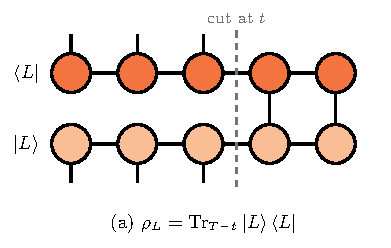
\includegraphics[width=0.92\textwidth]{rdm_rtm_a.pdf}\\[1.4ex]
      {\small pairs a state with \textbf{its own conjugate}\\[0.3ex]
        $\Rightarrow$ Hermitian, positive}
    \end{column}
    \begin{column}{0.48\textwidth}
      \centering
      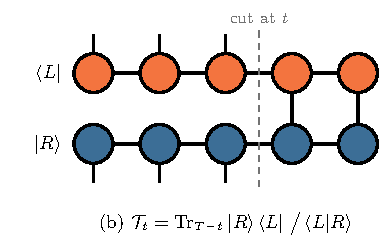
\includegraphics[width=0.92\textwidth]{rdm_rtm_b.pdf}\\[1.4ex]
      {\small pairs the \textbf{two distinct fixed points}
        $\bra{L}$, $\ket{R}$\\[0.3ex]
        $\Rightarrow$ non-Hermitian, complex eigenvalues allowed}
    \end{column}
  \end{columns}
  \vfill
\end{frame}

\begin{frame}{Backup D2 --- Entanglement through the SVD}
  \begin{columns}[c]
    \begin{column}{0.44\textwidth}
      \centering
      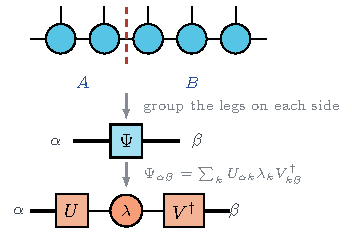
\includegraphics[width=\textwidth]{svd_schmidt.pdf}
    \end{column}
    \begin{column}{0.54\textwidth}
      \[
        \ket{\Psi} = \sum_{ij}\Psi_{ij}\,\ket{i}_A\ket{j}_B
      \]
      \vspace{-1.0em}
      \begin{center}\small\color{ink!70}
        across the cut the state is a matrix
      \end{center}
      \vspace{0.3em}
      \[
        \Psi = U\lambda V^{\dagger}
        \quad\Longrightarrow\quad
        \ket{\Psi} = \sum_k \lambda_k \ket{v_k}_A\ket{w_k}_B
      \]
      \vspace{-1.0em}
      \begin{center}\small\color{ink!70}
        the \textbf{Schmidt decomposition}
      \end{center}
    \end{column}
  \end{columns}
  \vfill
  \begin{center}
    $\displaystyle S = -\Tr\big(\rho_A\log\rho_A\big)
      = -\sum_k \lambda_k^{2}\log\lambda_k^{2}$
    \quad{\small\color{ink!70} the $\lambda_k^{2}$ are the eigenvalues
      of $\rho_A$}
  \end{center}
  \vfill
  \idea{one set of numbers ranks the directions \emph{and} carries the
    entanglement\\ $\Rightarrow$ truncation $=$ keep the largest $\lambda_k$}
\end{frame}

\begin{frame}{Backup D3 --- the Local RDM Reduction}
  \begin{center}
    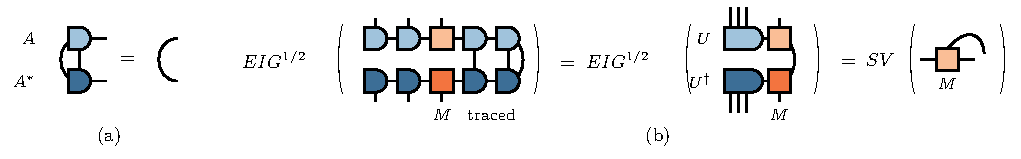
\includegraphics[width=\textwidth]{rdm_trunc_row.pdf}
  \end{center}
  \vspace{0.4em}
  {\small
    \begin{itemize}\setlength{\itemsep}{0.35em}
      \item mixed canonical form: away from the cut every tensor meets \textbf{its own
              conjugate} and contracts to the identity --- panel (a)
      \item the traced block then disappears column by column and the open block groups into
            one isometry per side: $\rho_B = U_B\,M_A\,U_B^{\dagger}$ with
            $U_B^{\dagger}U_B=\mathbb{1}$ $\Rightarrow$
            $\mathrm{eig}(\rho_B)=\mathrm{eig}(M_A)$, a $\chi\times\chi$ object ---
            the exponentially large matrix is never built
      \item eigenvalues $=$ squared singular values of $M$, one-to-one $\Rightarrow$ keep the
            $\chi'$ largest (optimal; error $=$ discarded weight)
    \end{itemize}}
\end{frame}

\begin{frame}{Backup D4 --- RTM Truncation: the Same Reduction, Different Isometries}
  \begin{center}
    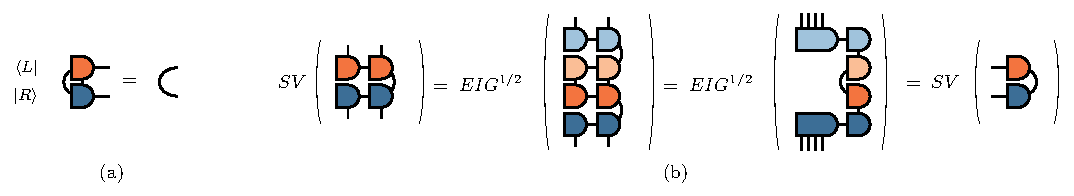
\includegraphics[width=0.96\textwidth]{rtm_trunc_row.pdf}
  \end{center}
  {\small
    \begin{itemize}\setlength{\itemsep}{0.25em}
      \item generalised canonical form: each $\bra{L}$ tensor is paired with
            the corresponding $\ket{R}$ tensor --- the isometries on the two
            sides differ
      \item local reduction: $\;\tau_B = U_B\, M_A\, V_B$ with
            $U_B\neq V_B^{\dagger}$ $\Rightarrow$ eigenvalues NOT preserved, but
            $\mathrm{sv}(\tau_B)=\mathrm{sv}(M_A)$
      \item so we truncate the $\chi\times\chi$ environment on its
            \textbf{singular values}; for the RTM these are no longer one-to-one
            with the eigenvalues (non-Hermitian) --- no variational bound
    \end{itemize}}
\end{frame}

\begin{frame}{Backup D5 --- How the Iteration Stops}
  \begin{columns}[c]
    \begin{column}{0.42\textwidth}
      {\small
        \begin{enumerate}\setlength{\itemsep}{0.4em}
          \item $\mathrm{d}s$ $=$ change in the singular values of the
                temporal state between successive iterations --- the convergence
                criterion in the code
          \item stop when $\mathrm{d}s$ falls below tolerance, or after
                $150$ iterations without improvement
          \item RTM hits a noise floor (no-improvement stop) while RDM
                converges --- yet both return the same leading eigenvalue to
                better than 1 part in $10^{4}$
        \end{enumerate}}
    \end{column}
    \begin{column}{0.56\textwidth}
      \centering
      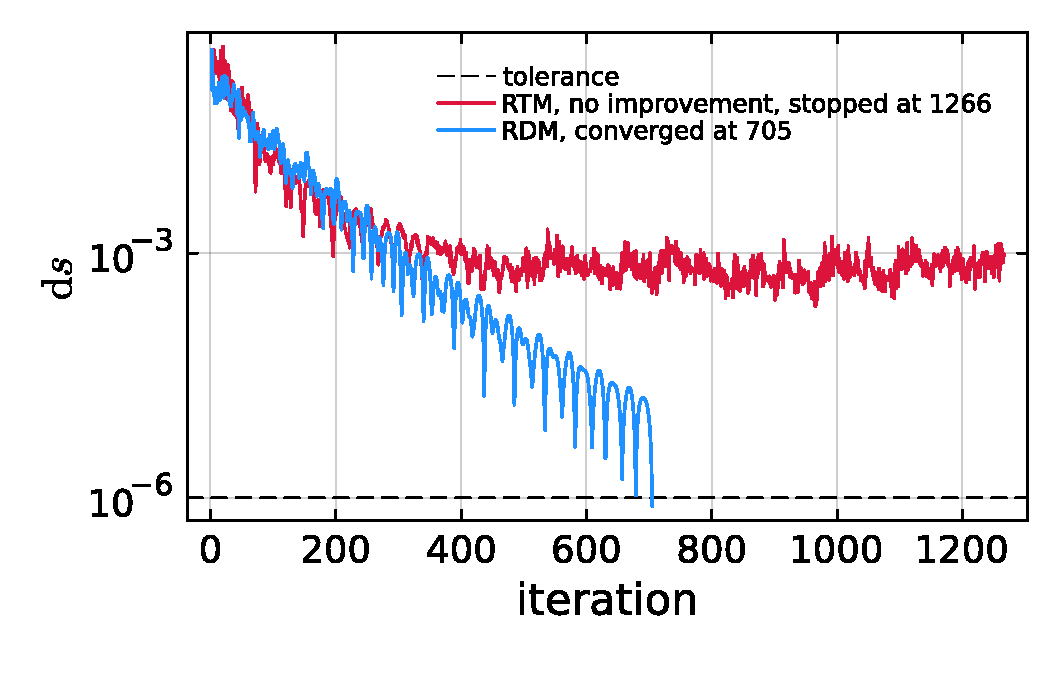
\includegraphics[width=\textwidth,height=0.7\textheight,keepaspectratio]{res_conv.pdf}
    \end{column}
  \end{columns}
\end{frame}

\begin{frame}{Backup D6 --- Why the Windows End}
  \vspace{-0.2em}
  \begin{center}\small
    the two routes need different things from $\E$:\\[0.2ex]
    \tint{routeL}{\parbox{0.40\textwidth}{\centering \textbf{eigenvalues}:
        {\footnotesize second-order accurate}}}\quad
    \tint{routeV}{\parbox{0.40\textwidth}{\centering \textbf{eigenvectors}:
        {\footnotesize sensitivity $\propto 1/\text{gap}$}}}
  \end{center}
  \begin{center}\small
    emergent dual unitarity shrinks the gaps $\Rightarrow$ the
    eigenvectors go first\\[0.2ex]
    {\footnotesize\color{ink!70} first rejected run at
      $T = 18,\ 11,\ 7,\ 3.5$ as $p$ goes $0 \to 0.5$}
  \end{center}
  \begin{center}\footnotesize\color{ink!70}
    is that just a \emph{closing} gap? --- exact diagonalisation, no
    truncation, no tensor networks:
  \end{center}
  \vspace{-0.4em}
  {\centering\small
    \setlength{\tabcolsep}{9pt}\renewcommand{\arraystretch}{1.05}%
    \begin{tabular}{@{}ccccc@{}}
      \toprule
      $p$   & $T$   & dimension & $|\mu_0-\mu_1|$ & $\mathrm{cond}(V)$ \\
      \midrule
      $0$   & $3.5$ & $2187$    & $0.21$          & $3.0\times10^{2}$  \\
      $0.1$ & $1.5$ & $2197$    & $0.30$          & $2.2\times10^{11}$ \\
      $0.3$ & $1.5$ & $2197$    & $0.19$          & $2.1\times10^{10}$ \\
      $0.5$ & $1.5$ & $2197$    & $0.14$          & $9.6\times10^{9}$  \\
      \bottomrule
    \end{tabular}\par}
  \vspace{0.1em}
  \idea{the gap barely moves; the eigenvector \emph{basis} degenerates by
    $7$--$9$ orders}
\end{frame}

% ---- backup: the block method ---------------------------------------------------

\slidesection{backup $\cdot$ the block method}
\begin{frame}{Backup E1 --- the Block Iteration, Step by Step}
  \small
  \textbf{Algorithm (App.~F, Alg.~1):} the $k$ dominant eigenpairs of $\E$
  \begin{enumerate}\setlength{\itemsep}{0.35em}
    \item $\ket{R_j},\,\bra{L_j} \gets$ random complex tMPS, \ $j=1,\dots,k$
    \item \textbf{apply:}\quad
          $\ket{\tilde R_j} \gets \mathrm{truncate}_\chi(\E\ket{R_j})$,\qquad
          $\bra{\tilde L_j} \gets \mathrm{truncate}_\chi(\bra{L_j}\E)$
    \item \textbf{project:}\quad
          $S_{ij}=\braket{L_i}{R_j}$,\qquad
          $M_{ij}=\bra{L_i}\E\ket{R_j}$
    \item solve $Mv=\theta Sv$ (via $\operatorname{pinv}(S)M$) for Ritz
          values $\theta_1,\dots,\theta_k$ and coefficients $V$, $U$
    \item \textbf{separate:}\quad
          $\ket{R_j} \gets \mathrm{truncate}_\chi\big(\textstyle\sum_i
            V_{ij}\ket{\tilde R_i}\big)$, \ analogously $\bra{L_j}$ with $U$
    \item normalise; repeat 2--5 until the leading Ritz values stop
          changing within tolerance
  \end{enumerate}
\end{frame}

\begin{frame}{Backup E2 --- the Block Method against Exact Diagonalisation}
  \vfill
  \begin{center}\small
    at short times the rotated column fits as a dense array: diagonalise
    it with\\ no state truncation and no projection onto a block, and compare
  \end{center}
  \vfill
  {\centering\small
    \setlength{\tabcolsep}{7pt}\renewcommand{\arraystretch}{1.2}%
    \begin{tabular}{@{}lcccc@{}}
      \toprule
      operator                    & dim.\  & exact $|\mu_0|,\,|\mu_1|$ & error               & stopped on     \\
      \midrule
      critical Ising, $T=1.5$     & $27$   & $0.9048,\;0.8373$         & $2.5\times10^{-12}$ & tolerance      \\
      critical Ising, $T=2$       & $81$   & $0.9129,\;0.8702$         & $2.3\times10^{-7}$  & no improvement \\
      ANNNI-type $p=0.1$, $T=1.5$ & $2197$ & $0.9405,\;0.9082$         & $1.2\times10^{-7}$  & no improvement \\
      \bottomrule
    \end{tabular}\par}
  \vspace{0.3em}
  \begin{center}\footnotesize\color{ink!70}
    $\delta t = 0.5$, no cooling sites; none of the three reaches the bond cap
  \end{center}
  \vfill
  \idea{the reduced eigenproblem adds no measurable error ---\\
    the accuracy is set by \emph{convergence}, not by the projection}
  \vfill
\end{frame}

% ---- backup: the fits ---------------------------------------------------

\slidesection{backup $\cdot$ the fits}
\begin{frame}{Backup F1 --- Why the Spectral $c$ Sits Below $\tfrac12$ at $p=0$}
  \begin{columns}[t]
    \begin{column}{0.46\textwidth}
      {\centering \textbf{1. the fit truncates the expansion}\par}
      \[
        \frac{\operatorname{Im}\lambda_0}{T}
        = a_0 - \frac{\pi}{T}
        \underbrace{-\,\frac{\pi c}{24\,v\,T^{2}}}_{\text{$c$ from here}}
        \;\underbrace{+\;\frac{D}{T^{4}}}_{\text{dropped}}
        +\;\ldots
      \]
      {\centering\small dropped term $=\;D/T^{3}$ in $\operatorname{Im}\lambda_0$\par}
      \idea{restoring it: $90\%\to97\%$ of the predicted coefficient}
    \end{column}
    \begin{column}{0.52\textwidth}
      {\centering \textbf{2. the regulator $\beta_0$ is finite}\par}
      \centering
      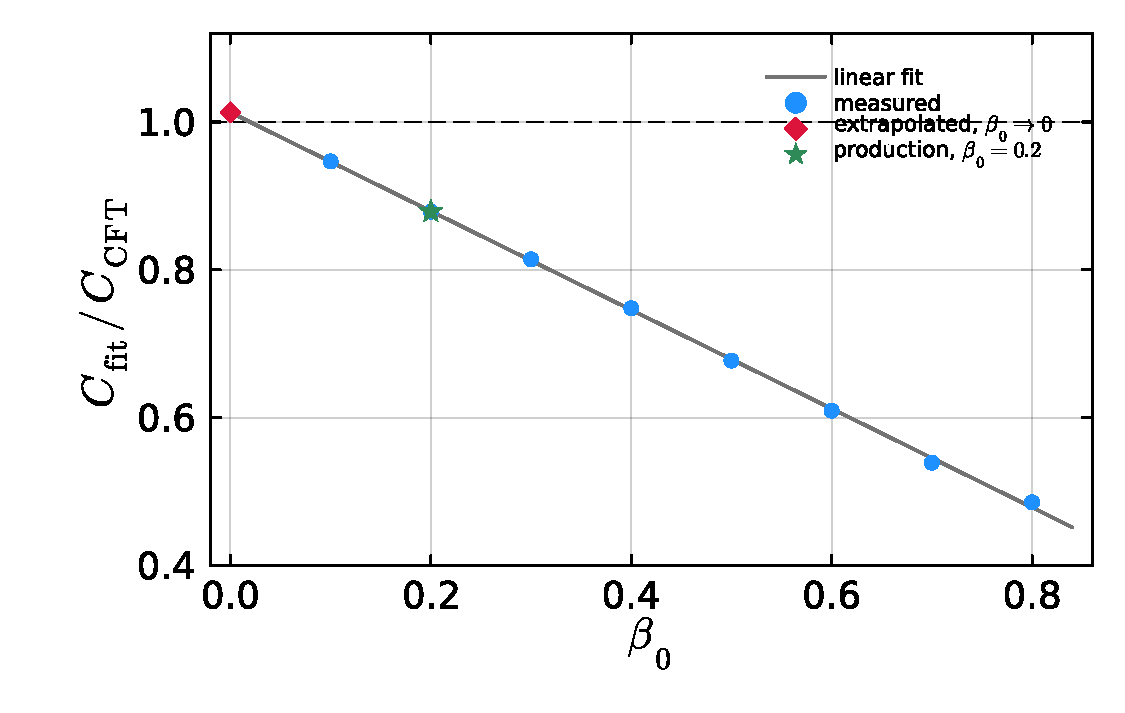
\includegraphics[width=\textwidth]{res_beta0.pdf}
    \end{column}
  \end{columns}
\end{frame}

\begin{frame}{Backup F2 --- Why the Real Part Cannot Measure $c$}
  \begin{columns}[c]
    \begin{column}{0.40\textwidth}
      \[
        \operatorname{Re}S_2 = s_0 + \frac{c}{8}\,W
        + a\,w^{-1/2}
      \]
    \end{column}
    \begin{column}{0.58\textwidth}
      \centering
      
\includegraphics[width=\textwidth]{res_re_c.pdf}
    \end{column}
  \end{columns}
\end{frame}

\begin{frame}{Backup F3 --- Four Boundary Condition Pairs}
  \begin{columns}[c]
    \begin{column}{0.28\textwidth}
      \begin{center}
        a \textbf{tower} $=$ the set of boundary operators a given pair of
        boundary conditions allows, and their descendants
      \end{center}
    \end{column}
    \begin{column}{0.70\textwidth}
      \centering
      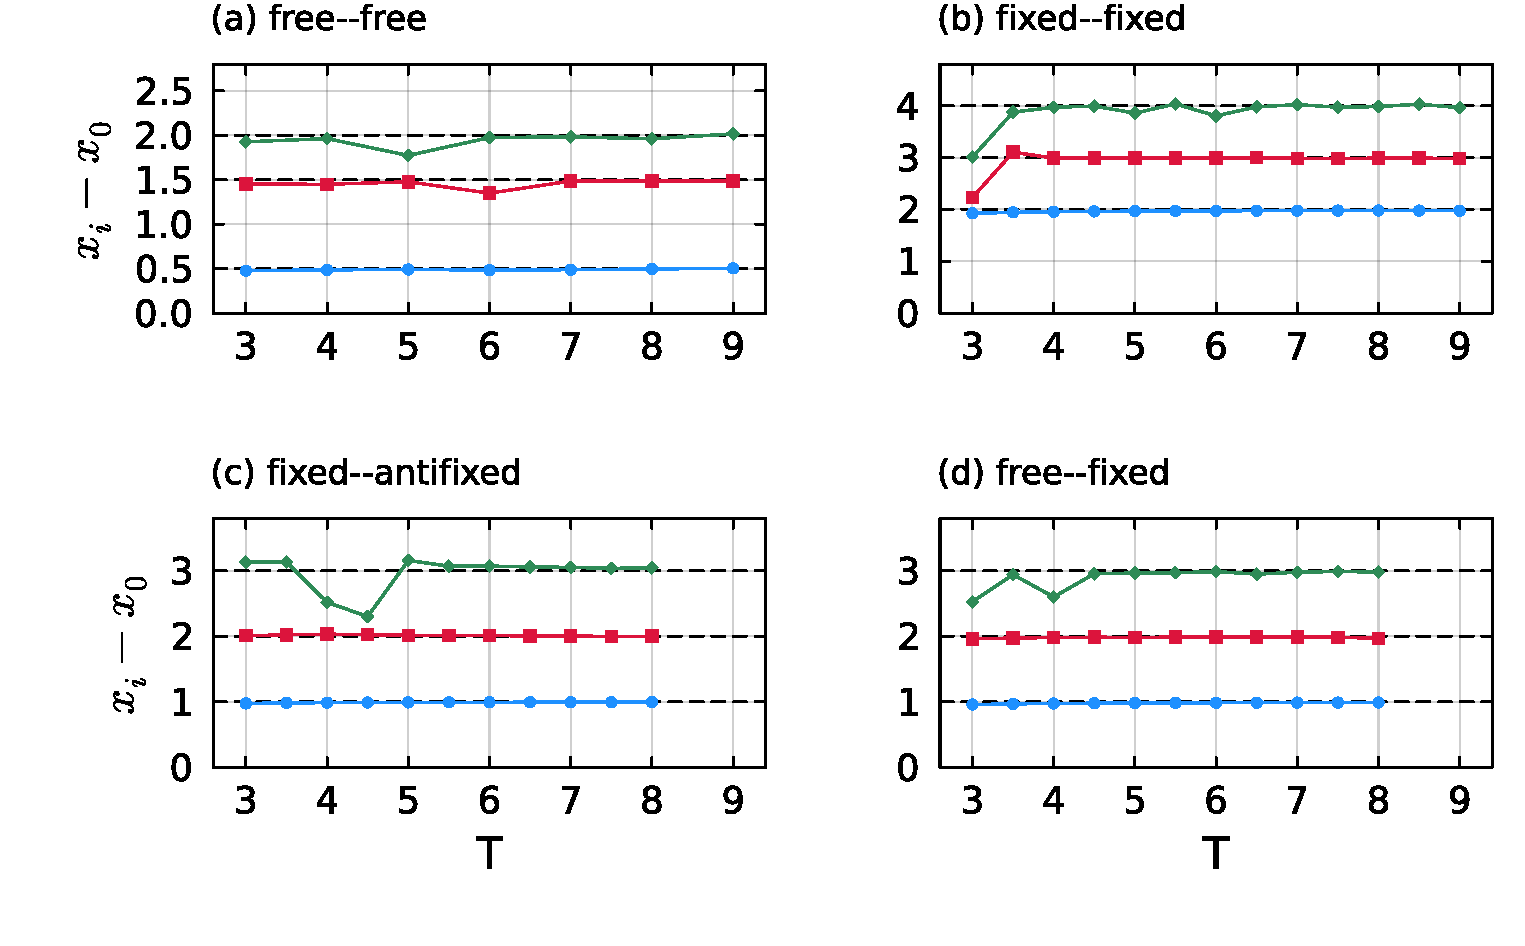
\includegraphics[width=\textwidth]{res_bc_pairs.pdf}
    \end{column}
  \end{columns}
\end{frame}

% restore the counter so \inserttotalframenumber = number of MAIN frames
\setcounter{framenumber}{\value{finalframe}}

\end{document}
